% =====================================================================
%  Algoritmo Memético para CVRP — Reporte académico
%  MIAAD UACJ · Optimización Inteligente · Mtro. Raúl Gibrán Porras
%  Alumno: Javier Augusto Rebull Saucedo (matrícula 263483)
%  Mayo 2026
%
%  Compilación recomendada (Overleaf):
%      pdflatex → biber → pdflatex → pdflatex
% =====================================================================
\documentclass[12pt,a4paper]{article}

\usepackage[spanish]{babel}
\usepackage[utf8]{inputenc}
\usepackage[T1]{fontenc}
\usepackage[margin=2.5cm]{geometry}
\usepackage{amsmath, amssymb}
\usepackage{algorithm2e}
\usepackage{booktabs}
\usepackage{tabularx}        % tablas con columnas X que se ajustan solas
\usepackage{array}           % requerido por >{\raggedright\arraybackslash}X
\usepackage{float}           % activa la opción [H] para floats fijos
\usepackage{graphicx}
\usepackage{xcolor}
\usepackage{caption}
\usepackage{subcaption}
\usepackage{csquotes}
\usepackage{microtype}       % micro-ajustes de espaciado contra overflow
\usepackage{seqsplit}        % rompe identificadores largos en \texttt
\usepackage[backend=biber, style=numeric, sorting=none]{biblatex}
\usepackage{xurl}            % URLs largas se rompen donde sea (debe ir antes de hyperref)
\usepackage{hyperref}

% Para nombres tipo `aceptaciones_no_mejorantes_tabu`:
% atajo \pyid{...} = \texttt{} pero con guión bajo permitido y posibilidad
% de romper línea en cada caracter. Usado en prosa para identificadores largos.
\newcommand{\pyid}[1]{\texttt{\seqsplit{#1}}}

% Caja destacada para llamadas de atención (sitio web, demo, etc.).
\newcommand{\callout}[2]{%
  \begin{center}
  \fcolorbox{teal!50}{teal!7}{\begin{minipage}{0.92\linewidth}\vspace{0.3em}
    \textbf{\color{teal!70!black}#1}\par\vspace{0.4em}#2\vspace{0.3em}
  \end{minipage}}
  \end{center}}

\hypersetup{
    colorlinks=true,
    linkcolor=black,
    citecolor=teal,
    urlcolor=teal,
    pdftitle={Algoritmo Memetico para CVRP — MIAAD UACJ},
    pdfauthor={Javier Augusto Rebull Saucedo}
}

\graphicspath{{./figures/}}
\addbibresource{references.bib}

% --- Portada ---
\title{
    \vspace{-2cm}
    \large Universidad Autónoma de Ciudad Juárez \\
    \large Maestría en Inteligencia Artificial y Analítica de Datos (MIAAD) \\
    \large Optimización Inteligente \\
    \vspace{1cm}
    \Huge \textbf{Algoritmo Memético para el Problema de Enrutamiento de Vehículos con Capacidad (CVRP)} \\
    \vspace{0.5cm}
    \large Fusión de Algoritmo Genético y Búsqueda Tabú para optimización combinatoria
}

\author{
    \textbf{Javier Augusto Rebull Saucedo} \\
    Matrícula 263483 \\
    \vspace{0.3cm}
    \textit{Profesor:} Mtro. Raúl Gibrán Porras Alaniz
}

\date{Mayo de 2026}

% =====================================================================
\begin{document}
\maketitle
\thispagestyle{empty}

\begin{abstract}
Se implementa desde cero un Algoritmo Memético que combina un Algoritmo Genético (exploración global) con Búsqueda Tabú (intensificación local) para resolver el Capacitated Vehicle Routing Problem (CVRP). El cromosoma sigue la representación \emph{Giant Tour} y se decodifica con un \emph{Split} capacitado; la cruza es \emph{Order Crossover} (OX) y la búsqueda local opera por \emph{swaps} con tenencia y aspiración. Se evalúa en tres escenarios de estrés ($N{=}50,Q{=}100$; $N{=}100,Q{=}30$; $N{=}75,Q{=}200$) con multi-seed para validez estadística. Resultados, código y reporte son reproducibles bit a bit.
\end{abstract}

\newpage
\tableofcontents
\newpage

% --- Secciones ---
\section{Introducción}
\label{sec:introduccion}

El \textbf{Problema de Enrutamiento de Vehículos con Capacidad} (\emph{Capacitated Vehicle Routing Problem}, CVRP) es uno de los problemas de optimización combinatoria más estudiados desde su formulación original por Dantzig y Ramser \cite{dantzig1959truck}. Su relevancia industrial es enorme: distribución logística, recolección de residuos, abastecimiento de cajeros automáticos, ruteo de paquetería de última milla. La dificultad teórica también lo es: el CVRP es \textbf{NP-duro} en sentido fuerte, por lo que los métodos exactos sólo escalan hasta unas pocas decenas de clientes con cómputo razonable.

En la práctica, el estado del arte para instancias medianas y grandes son las \textbf{metaheurísticas}, en particular las que combinan exploración global y explotación local. Los \emph{Algoritmos Genéticos} (GA) \cite{holland1975adaptation} sobresalen para barrer el espacio de soluciones en regiones diversas mediante cruza, pero pierden eficiencia al pulir soluciones cercanas a un óptimo local. La \emph{Búsqueda Tabú} (TS) de Glover \cite{glover1986future} es exactamente lo opuesto: brilla afinando soluciones, pero depende del punto inicial. El \emph{Algoritmo Memético} \cite{moscato1989evolution} fusiona ambos paradigmas: el GA decide \emph{dónde} buscar y la búsqueda local decide \emph{cómo} explotar esa región.

\subsection*{Aporte de este trabajo}

Este reporte documenta la implementación \textbf{desde cero} (sin librerías de optimización VRP externas) de un Algoritmo Memético GA + Tabú aplicado a tres escenarios deterministas del CVRP, con multi-seed para validez estadística y reproducibilidad bit-a-bit. Se hace énfasis en:

\begin{itemize}
    \item Una implementación clara y modular en Python puro con pruebas unitarias.
    \item La discusión de trade-offs entre presión selectiva, intensificación local y diversidad poblacional.
    \item La presentación visual sobria de los resultados en un reporte LaTeX y en un sitio web estático Nuxt.
\end{itemize}

El código completo, con instrucciones de reproducción, está disponible en \url{https://github.com/jrebull/MIAAD_SmartOpti_memetic}.

\callout{Sitio interactivo del proyecto: \href{https://miaadmemetic.netlify.app}{\nolinkurl{miaadmemetic.netlify.app}}}{%
Toda esta investigación tiene una versión \emph{viva} en línea. El sitio expone:%
\begin{itemize}\setlength\itemsep{0pt}
  \item \textbf{Dashboard de resultados} — los cuatro escenarios con sus métricas, gráficas de convergencia y mapas de rutas pre\-calculados.
  \item \textbf{Playground Pyodide} — el mismo paquete \pyid{memetico\_cvrp} ejecut\'andose dentro del navegador del visitante v\'ia WebAssembly. Permite ajustar hiperpar\'ametros con \emph{sliders} y observar la convergencia generaci\'on por generaci\'on en vivo, sobre cualquiera de los cuatro escenarios.
  \item \textbf{Visor del c\'odigo fuente} de los siete m\'odulos del paquete con \emph{syntax highlighting} y descripci\'on de cada uno (\href{https://miaadmemetic.netlify.app/codigo}{/codigo}).
  \item \textbf{Reproducibilidad documentada}: instrucciones de un solo comando (\texttt{make ci}) para regenerar todos los resultados desde cero.
\end{itemize}}

\section{Marco teórico}
\label{sec:marco}

\subsection{Formulación del CVRP}

Sea $V = \{0, 1, \ldots, N\}$ el conjunto de nodos, donde $0$ representa el depósito y $\{1, \ldots, N\}$ los clientes. Cada cliente $i$ tiene una demanda $q_i > 0$. La flota es homogénea con $K$ vehículos idénticos, cada uno con capacidad $Q$. La distancia euclidiana entre los nodos $i$ y $j$ es:
$$d_{ij} = \sqrt{(x_i - x_j)^2 + (y_i - y_j)^2}.$$

Definimos las variables binarias $x_{ijk} = 1$ si el vehículo $k$ viaja directamente del nodo $i$ al nodo $j$, y $0$ en otro caso. La función objetivo a \textbf{minimizar} es:

\begin{equation}
\label{eq:cvrp}
f(S) = \sum_{k=1}^{K} \sum_{i=0}^{N} \sum_{j=0}^{N} d_{ij}\, x_{ijk}.
\end{equation}

Sujeta a las tres restricciones duras del CVRP:

\begin{enumerate}
    \item \textbf{Cobertura única.} Cada cliente $j \in \{1, \ldots, N\}$ es visitado exactamente una vez por exactamente un vehículo:
    $$\sum_{k=1}^{K} \sum_{i=0}^{N} x_{ijk} = 1 \quad \forall\, j \in \{1, \ldots, N\}.$$
    \item \textbf{Balance en el depósito.} Todo vehículo que sale del depósito vuelve al depósito:
    $$\sum_{j=1}^{N} x_{0jk} = \sum_{i=1}^{N} x_{i0k} \quad \forall\, k.$$
    \item \textbf{Capacidad.} La carga total de la ruta de cada vehículo no excede $Q$:
    $$\sum_{i=1}^{N} q_i \sum_{j=0}^{N} x_{ijk} \leq Q \quad \forall\, k.$$
\end{enumerate}

\subsection{Representación Giant Tour y decodificador Split}

Codificar directamente las $K$ rutas como un cromosoma es engorroso porque obliga a operadores genéticos sensibles a la cardinalidad de la flota. Una alternativa elegante es la representación \textbf{Giant Tour}: un cromosoma es una permutación $(\pi_1, \pi_2, \ldots, \pi_N)$ de los $N$ clientes, sin separadores de ruta. Un decodificador determinista —el algoritmo \emph{Split} capacitado— recorre la permutación de izquierda a derecha y abre una nueva ruta cada vez que la siguiente demanda desbordaría la capacidad del vehículo actual. Así, todo cromosoma representa unívocamente una solución factible (mientras ningún cliente individual exceda $Q$).

\subsection{Order Crossover (OX)}

Dado que el cromosoma es una permutación sin duplicados ni faltantes, los operadores clásicos de cruza (un punto, uniforme) no aplican. El \textbf{Order Crossover} (Davis, 1985) es el estándar para permutaciones:

\begin{algorithm}[H]
\SetAlgoLined
\caption{Order Crossover (OX)}
\KwIn{Padres $P_1, P_2$ permutaciones de longitud $N$}
\KwOut{Hijo $H$, permutación válida}
Elegir dos puntos de corte $i < j$ uniformemente en $[0, N-1]$\;
$H[i..j] \leftarrow P_1[i..j]$\;
$pos \leftarrow (j + 1) \bmod N$\;
\For{cada gen $g$ recorriendo $P_2$ desde $j+1$ con wrap-around}{
    \If{$g \notin H$}{
        $H[pos] \leftarrow g$\;
        $pos \leftarrow (pos + 1) \bmod N$\;
    }
}
\Return $H$\;
\end{algorithm}

\subsection{Búsqueda Tabú con tenencia y aspiración}

La Búsqueda Tabú \cite{glover1986future} es una metaheurística de búsqueda local que escapa de óptimos locales mediante una \emph{memoria de corto plazo} de movimientos recientes. Para CVRP usamos el operador de vecindad \emph{swap} (intercambio de dos posiciones del cromosoma). En cada iteración:

\begin{enumerate}
    \item Se muestrean $s$ vecinos por swap.
    \item Para cada uno se evalúa el costo y se chequea si el movimiento $(\min(c_a, c_b), \max(c_a, c_b))$ está en la lista tabú.
    \item Un movimiento tabú puede ser aceptado si cumple el \emph{criterio de aspiración}: mejora el mejor global histórico.
    \item Se acepta el mejor vecino válido —incluso si empeora— para forzar la salida de óptimos locales.
    \item El movimiento se prohíbe durante $T$ iteraciones (\emph{tenencia}).
\end{enumerate}

\subsection{Algoritmo Memético}

La integración GA + TS se hace por \textbf{aprendizaje individual} (educación de hijos). Tras cada cruza OX, con probabilidad $p_{tabu}$ el hijo se somete a una corrida corta de Búsqueda Tabú antes de incorporarse a la siguiente población.

\begin{algorithm}[H]
\SetAlgoLined
\caption{Algoritmo Memético GA + Tabú para CVRP}
\KwIn{Población inicial aleatoria de tamaño $\mu$, generaciones $G$, prob. tabú $p_t$}
\KwOut{Mejor cromosoma encontrado}
Inicializar población $P_0$ aleatoria\;
Evaluar $\mathrm{fit}(P_0)$ vía Split\;
$best \leftarrow \arg\min_{c \in P_0} \mathrm{fit}(c)$\;
\For{$g = 1, \ldots, G$}{
    $P_{g} \leftarrow \{best\}$ \tcp*[r]{Elitismo}
    \While{$|P_g| < \mu$}{
        $p_1 \leftarrow$ TorneoSel($P_{g-1}, k$)\;
        $p_2 \leftarrow$ TorneoSel($P_{g-1}, k$)\;
        $h \leftarrow$ OX$(p_1, p_2)$\;
        \If{$\mathrm{rand}() < p_t$}{
            $h \leftarrow$ Tabu$(h, \text{iter}, \text{ten}, s)$\;
        }
        $P_g \leftarrow P_g \cup \{h\}$\;
    }
    $best \leftarrow \arg\min_{c \in P_g} \mathrm{fit}(c)$\;
}
\Return $best$\;
\end{algorithm}

La \emph{mutación clásica} se omite (o se reduce a probabilidad $\approx 0$) porque la propia Tabú actúa como una "super-mutación inteligente" \cite{moscato1989evolution}: la diversificación dirigida por memoria sustituye con ventaja a la mutación aleatoria.

\section{Metodología}
\label{sec:metodologia}

\subsection{Implementación}

El sistema se desarrolla en Python 3.11+ con NumPy, sin recurrir a librerías de optimización VRP externas (OR-Tools, PyVRP, VRPy). Cada componente reside en un módulo independiente y testable de \texttt{src/memetico\_cvrp/}:

\begin{itemize}
    \item \texttt{data.py} — Generación y carga de instancias (CSV deterministas).
    \item \texttt{distance.py} — Matriz de distancias precalculada vectorizada con \texttt{np.hypot}.
    \item \texttt{split.py} — Decodificador Giant Tour $\to$ rutas factibles.
    \item \texttt{genetic.py} — Población inicial, torneo, OX (con \texttt{np.random.Generator} inyectado).
    \item \texttt{tabu.py} — Búsqueda Tabú con muestreo de vecinos, tenencia y aspiración.
    \item \texttt{memetic.py} — Orquestador con elitismo y caché de fitness.
    \item \texttt{feasibility.py} — Validador blindado de soluciones.
\end{itemize}

La cobertura de pruebas unitarias supera el 80\% en los módulos críticos (\texttt{split}, \texttt{genetic}, \texttt{tabu}, \texttt{memetic}, \texttt{feasibility}), con tests parametrizados para distintos tamaños de instancia.

\subsection{Representación cromosómica: ejemplo}

Sea $N = 5$ clientes con demandas $q = (8, 4, 6, 3, 7)$ y capacidad $Q = 12$. Considérese el cromosoma $\pi = (1, 3, 4, 2, 5)$. El decodificador Split lo procesa así:

\begin{enumerate}
    \item Vehículo 1 abre en el depósito, toma cliente 1 (carga 8). Cliente 3 sumaría $8 + 6 = 14 > 12$: cierra ruta 1.
    \item Vehículo 2 toma cliente 3 (carga 6), luego cliente 4 (carga 9). Cliente 2 sumaría 13: cierra ruta 2.
    \item Vehículo 3 toma cliente 2 (carga 4), luego cliente 5 (carga 11): última ruta.
\end{enumerate}

Resultado: tres rutas $0 \to 1 \to 0$, $0 \to 3 \to 4 \to 0$, $0 \to 2 \to 5 \to 0$, con cargas $(8, 9, 11)$.

\subsection{Parámetros y diseño experimental}

Los hiperparámetros por escenario están versionados en \texttt{config/experiments.yaml} y siguen las recomendaciones del Apéndice A del plan brutal. Cada escenario se ejecuta con cinco semillas $\{2026, 2027, 2028, 2029, 2030\}$. La validación de factibilidad bloquea cualquier resultado infactible antes de persistirlo.

\subsection{Reproducibilidad}

Cada \emph{run} se serializa con metadatos completos: \texttt{git\_commit\_hash}, versión de Python y librerías, hash MD5 de la instancia y \emph{timestamp} UTC. El script \texttt{scripts/verificar\_reproducibilidad.py} re-ejecuta los runs en modo \emph{smoke} y compara contra los resultados anteriores. Dos ejecuciones del mismo \emph{seed} sobre la misma máquina producen resultados idénticos bit a bit.

\section{Diseño experimental}
\label{sec:experimentos}

\subsection{Escenarios}

Se evalúa el algoritmo memético sobre tres escenarios CVRP deterministas. Cada instancia se genera con una semilla específica y queda persistida en \pyid{data/raw/} junto con su archivo \pyid{.meta.json} (que registra parámetros, hash MD5 y \emph{timestamp}).

\begin{table}[H]
\centering
\small
\caption{Escenarios evaluados. Las semillas son las pactadas en el plan; cinco \emph{runs} por escenario.}
\begin{tabularx}{\linewidth}{>{\raggedright\arraybackslash}Xrr r >{\raggedright\arraybackslash}X}
\toprule
Escenario & $N$ & $Q$ & Semilla & \emph{Seeds} runs \\
\midrule
Caso 1 — Escala Media           & 50  & 100 & 20\,260\,201 & 2026--2030 \\
Caso 2 — Alta Densidad          & 100 & 30  & 20\,260\,202 & 2026--2030 \\
Caso 3 — Consolidación          & 75  & 200 & 20\,260\,203 & 2026--2030 \\
\bottomrule
\end{tabularx}
\end{table}

\subsection{Justificación del diseño multi-seed}

Reportar un único \emph{run} con suerte es engañoso: las metaheurísticas estocásticas pueden caer en óptimos locales muy distintos según el camino aleatorio. Reportar $n=5$ \emph{runs} permite distinguir entre el desempeño promedio y la dispersión, condición necesaria para hacer afirmaciones cuantitativas defendibles. En la sección de resultados se reportan media, mediana, mínimo, máximo y desviación estándar de cada métrica.

\subsection{Hiperparámetros por escenario}

\begin{table}[H]
\centering
\small
\caption{Hiperparámetros por escenario.}
\begin{tabular}{lrrrrrrr}
\toprule
Escenario & gen & pob & $k$ & $p_{\mathrm{tabu}}$ & iter\,Tabú & ten. & sample \\
\midrule
Caso 1 & 100 & 60 & 3 & 0.35 & 30 & 7 & 25 \\
Caso 2 & 150 & 80 & 3 & 0.45 & 35 & 9 & 35 \\
Caso 3 & 100 & 60 & 3 & 0.35 & 25 & 7 & 25 \\
\bottomrule
\end{tabular}
\end{table}

\paragraph{Por qué Caso 2 lleva más recursos.} El Caso 2 tiene $N = 100$ clientes (combinatorialmente $\sim 4 \times$ mayor que el Caso 1) y $Q = 30$ —es decir, requiere muchísimas rutas pequeñas, lo que multiplica la cantidad de configuraciones plausibles. Para no quedarse en óptimos locales tempranos, el algoritmo recibe mayor población, más generaciones, más probabilidad de aplicar Tabú y tenencia más larga.

\subsection{Entorno}

Todos los experimentos se ejecutan localmente (no se usa cómputo distribuido). El entorno está documentado en \pyid{requirements.txt}: NumPy 2.4, SciPy 1.17, pytest 9.0, Python 3.11+. La máquina de referencia es macOS 25.5 con Python 3.14.

\section{Resultados}
\label{sec:resultados}

\subsection{Resumen comparativo}

La tabla siguiente presenta los resultados agregados por escenario. Cada celda surge de cinco \emph{runs} con semillas distintas; se reporta el mejor costo histórico, la media, la desviación estándar, el número promedio de vehículos y el tiempo de cómputo.

\begin{table}[H]
\centering
\caption{Resumen de resultados por escenario}
\begin{tabular}{lrrrrrr}
\toprule
Escenario & Mejor & Media & Std & Veh. (med.) & Útil.\% & Tiempo (s) \\
\midrule
Instancia base del tutorial & 572.34 & 581.38 & 9.75 & 6.0 & 87.0 & 2.53 \\
Escala Media & 705.05 & 763.17 & 42.15 & 6.0 & 91.3 & 30.07 \\
Alta Densidad / Rutas Cortas & 3063.66 & 3099.86 & 18.21 & 38.0 & 89.7 & 310.66 \\
Rutas de Consolidación & 951.52 & 1035.93 & 43.42 & 4.0 & 93.0 & 31.37 \\
\bottomrule
\end{tabular}
\end{table}


\subsection{Convergencia y soluciones por escenario}

\paragraph{Caso 1 — Escala Media (\emph{N}=50, \emph{Q}=100).}

\begin{figure}[H]
    \centering
    \begin{subfigure}[b]{0.48\textwidth}
        \centering
        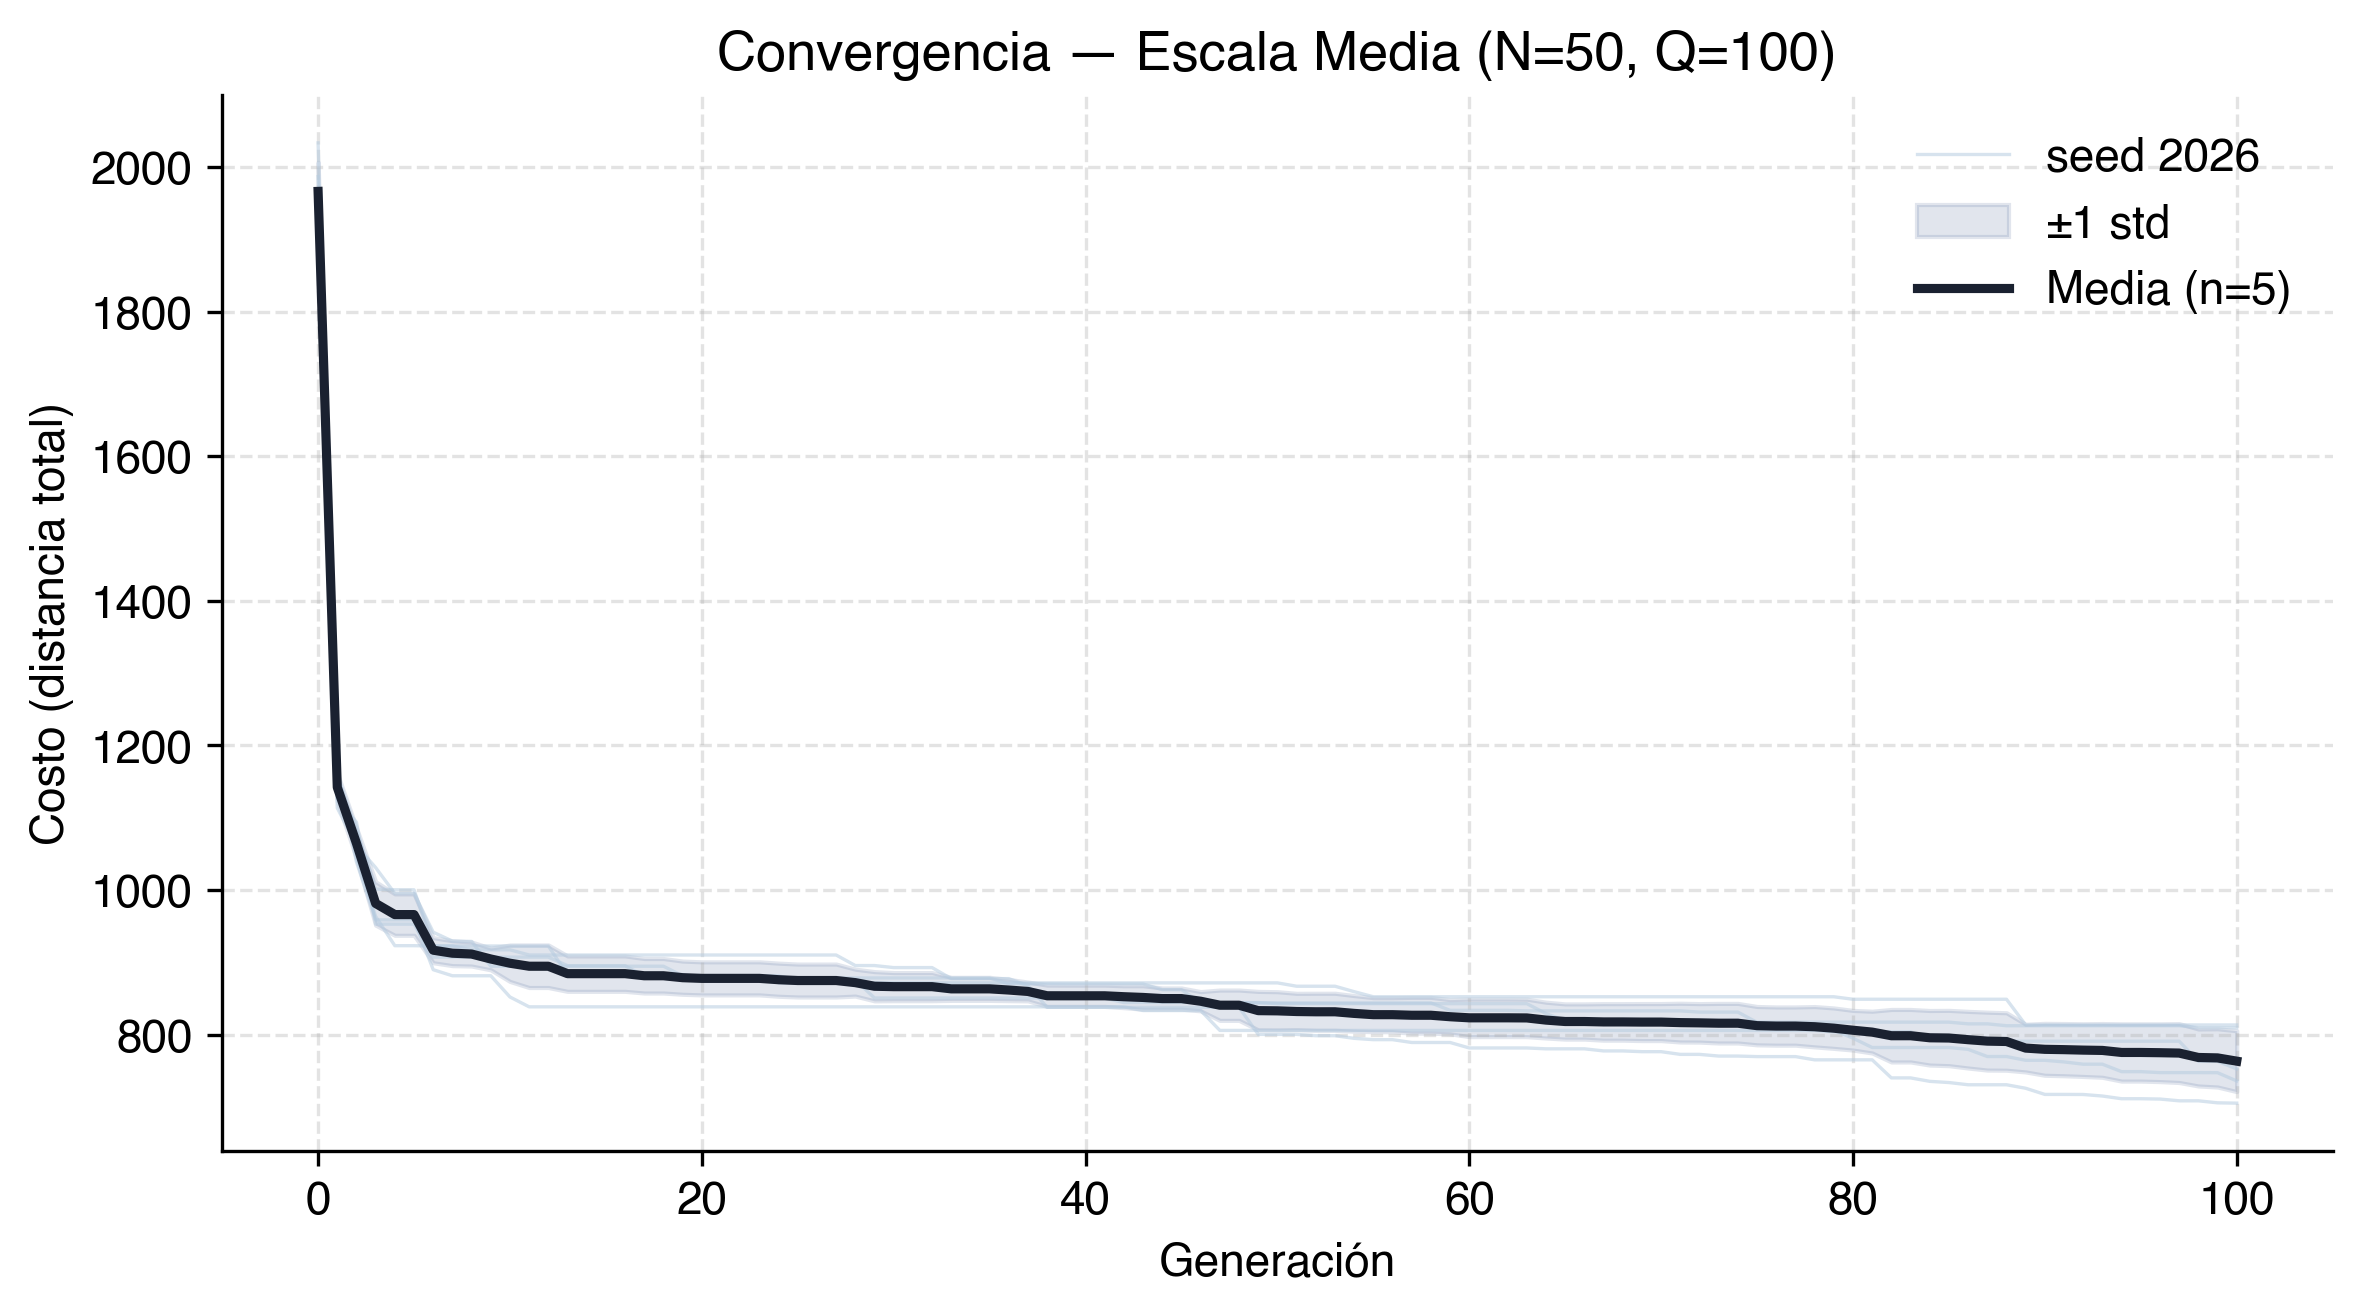
\includegraphics[width=\linewidth]{convergencia_caso_1.png}
        \caption{Convergencia (5 \emph{seeds}).}
        \label{fig:conv1}
    \end{subfigure}
    \hfill
    \begin{subfigure}[b]{0.48\textwidth}
        \centering
        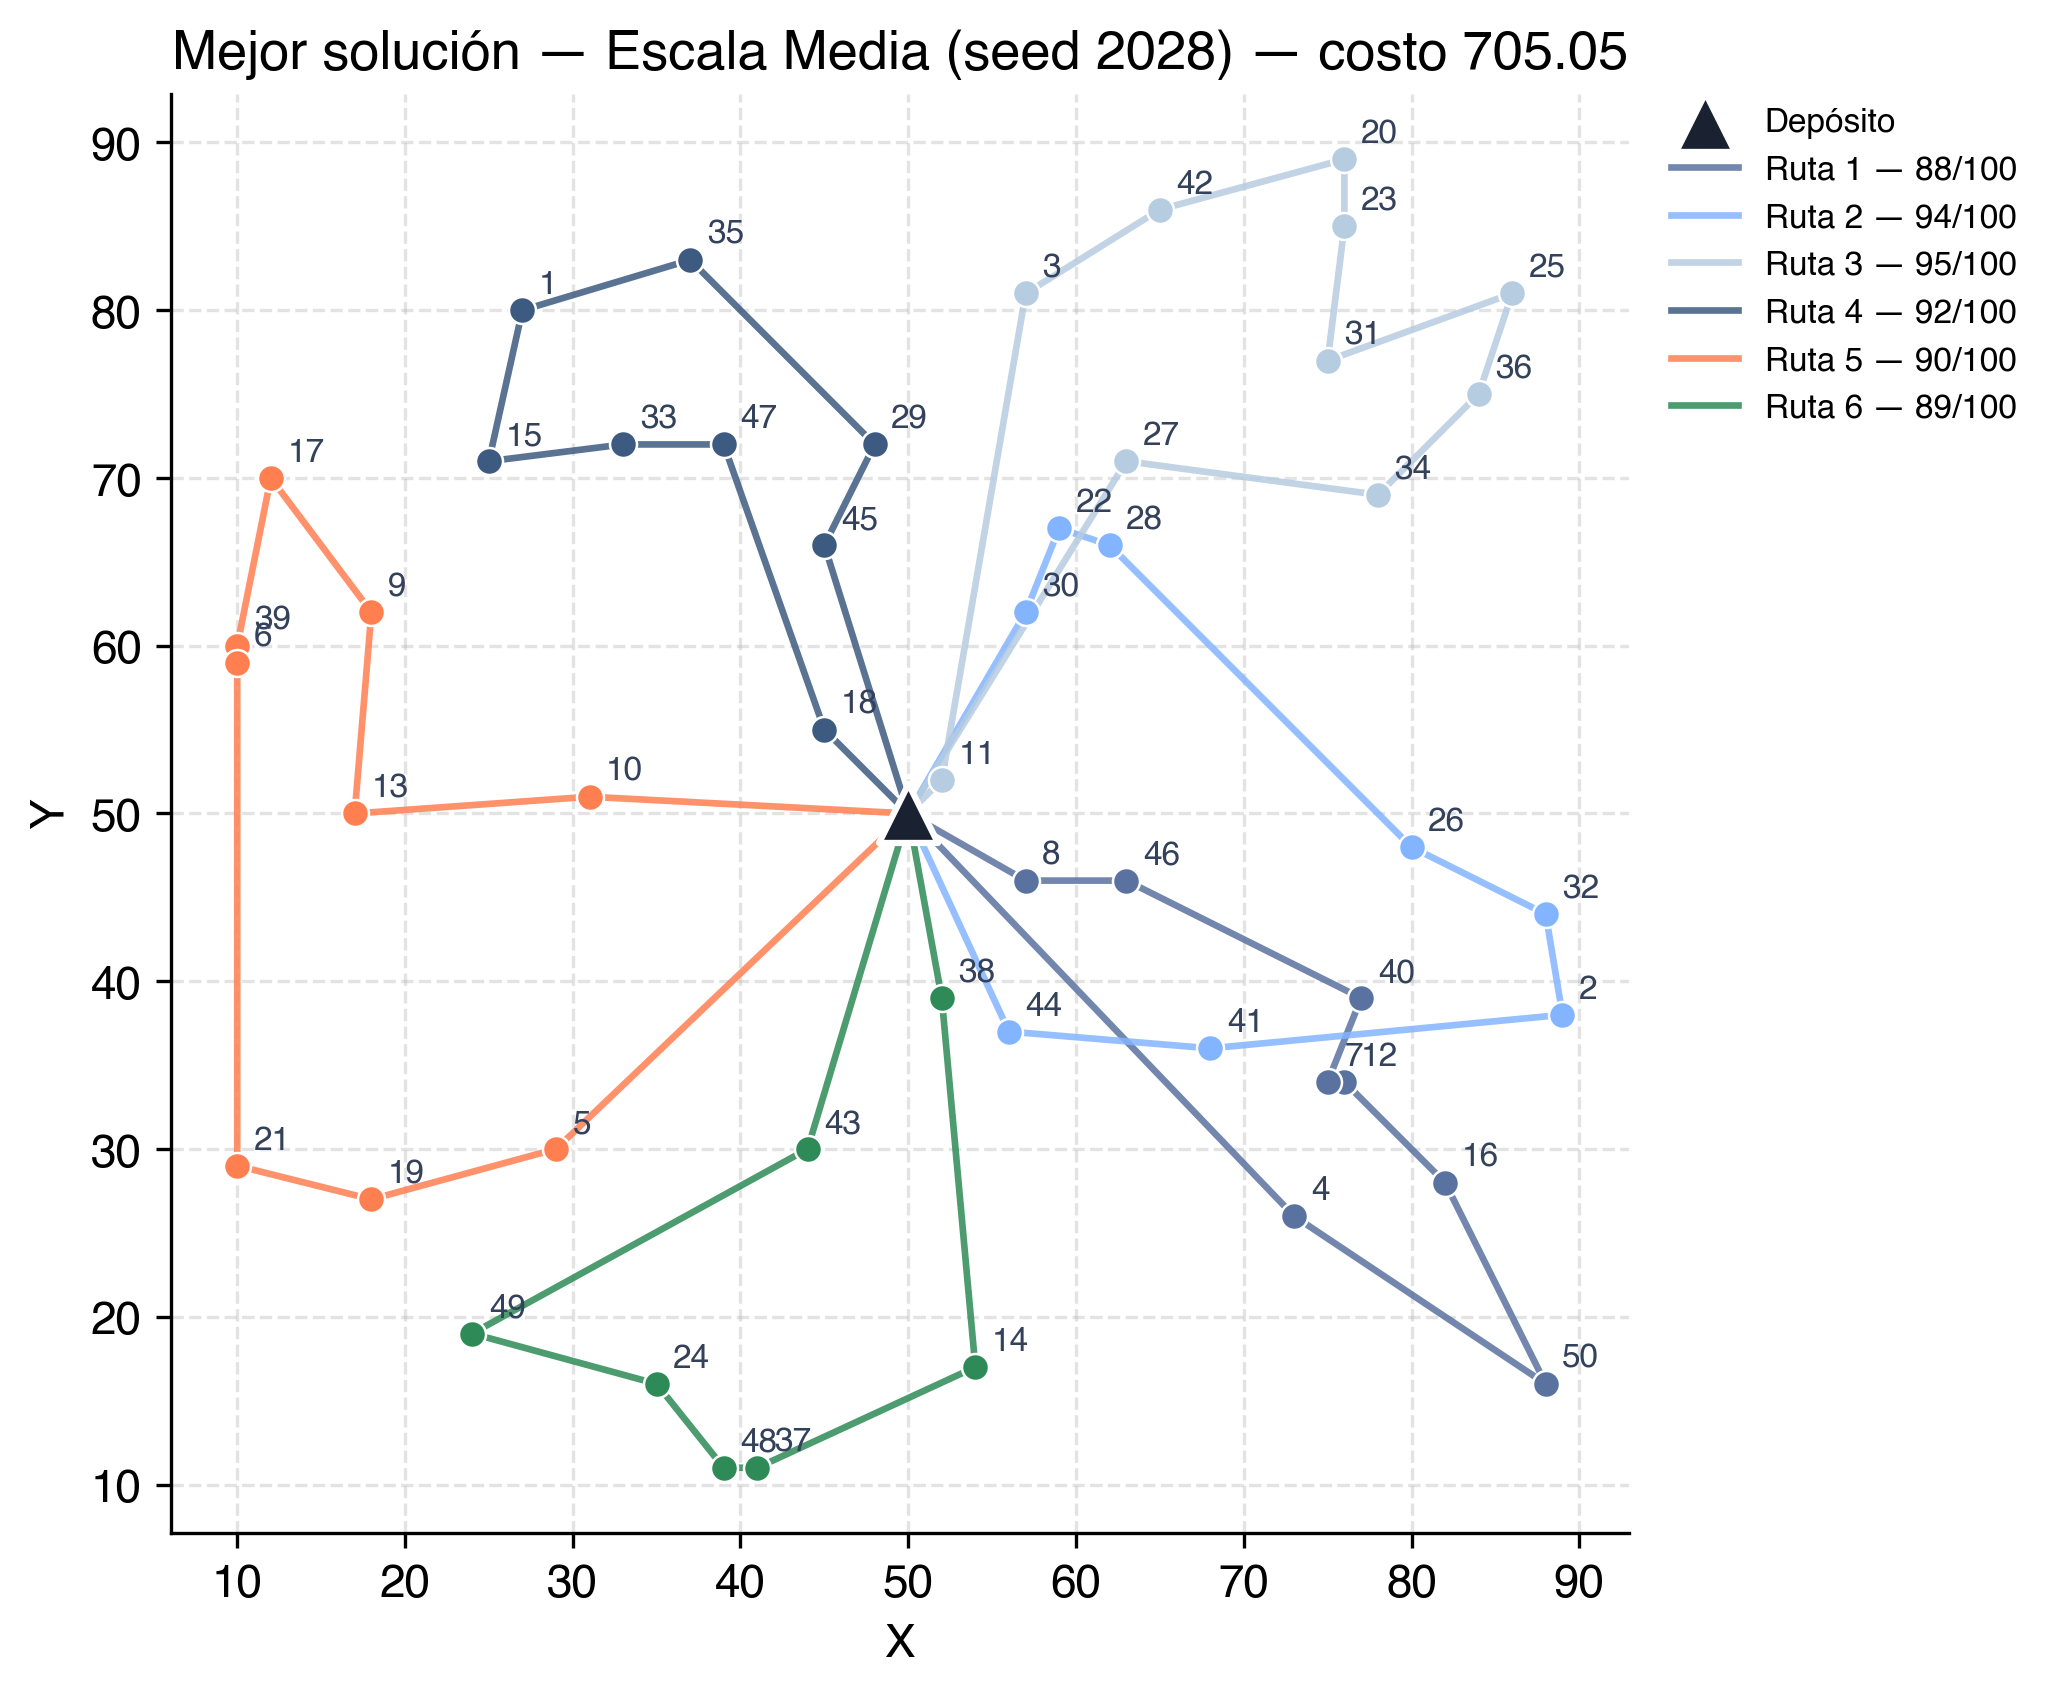
\includegraphics[width=\linewidth]{rutas_caso_1.png}
        \caption{Mejor solución encontrada.}
        \label{fig:rutas1}
    \end{subfigure}
    \caption{Caso 1. Histórico de convergencia y mapa de rutas del mejor \emph{run}.}
    \label{fig:caso1}
\end{figure}

\paragraph{Caso 2 — Alta Densidad / Rutas Cortas (\emph{N}=100, \emph{Q}=30).}

\begin{figure}[H]
    \centering
    \begin{subfigure}[b]{0.48\textwidth}
        \centering
        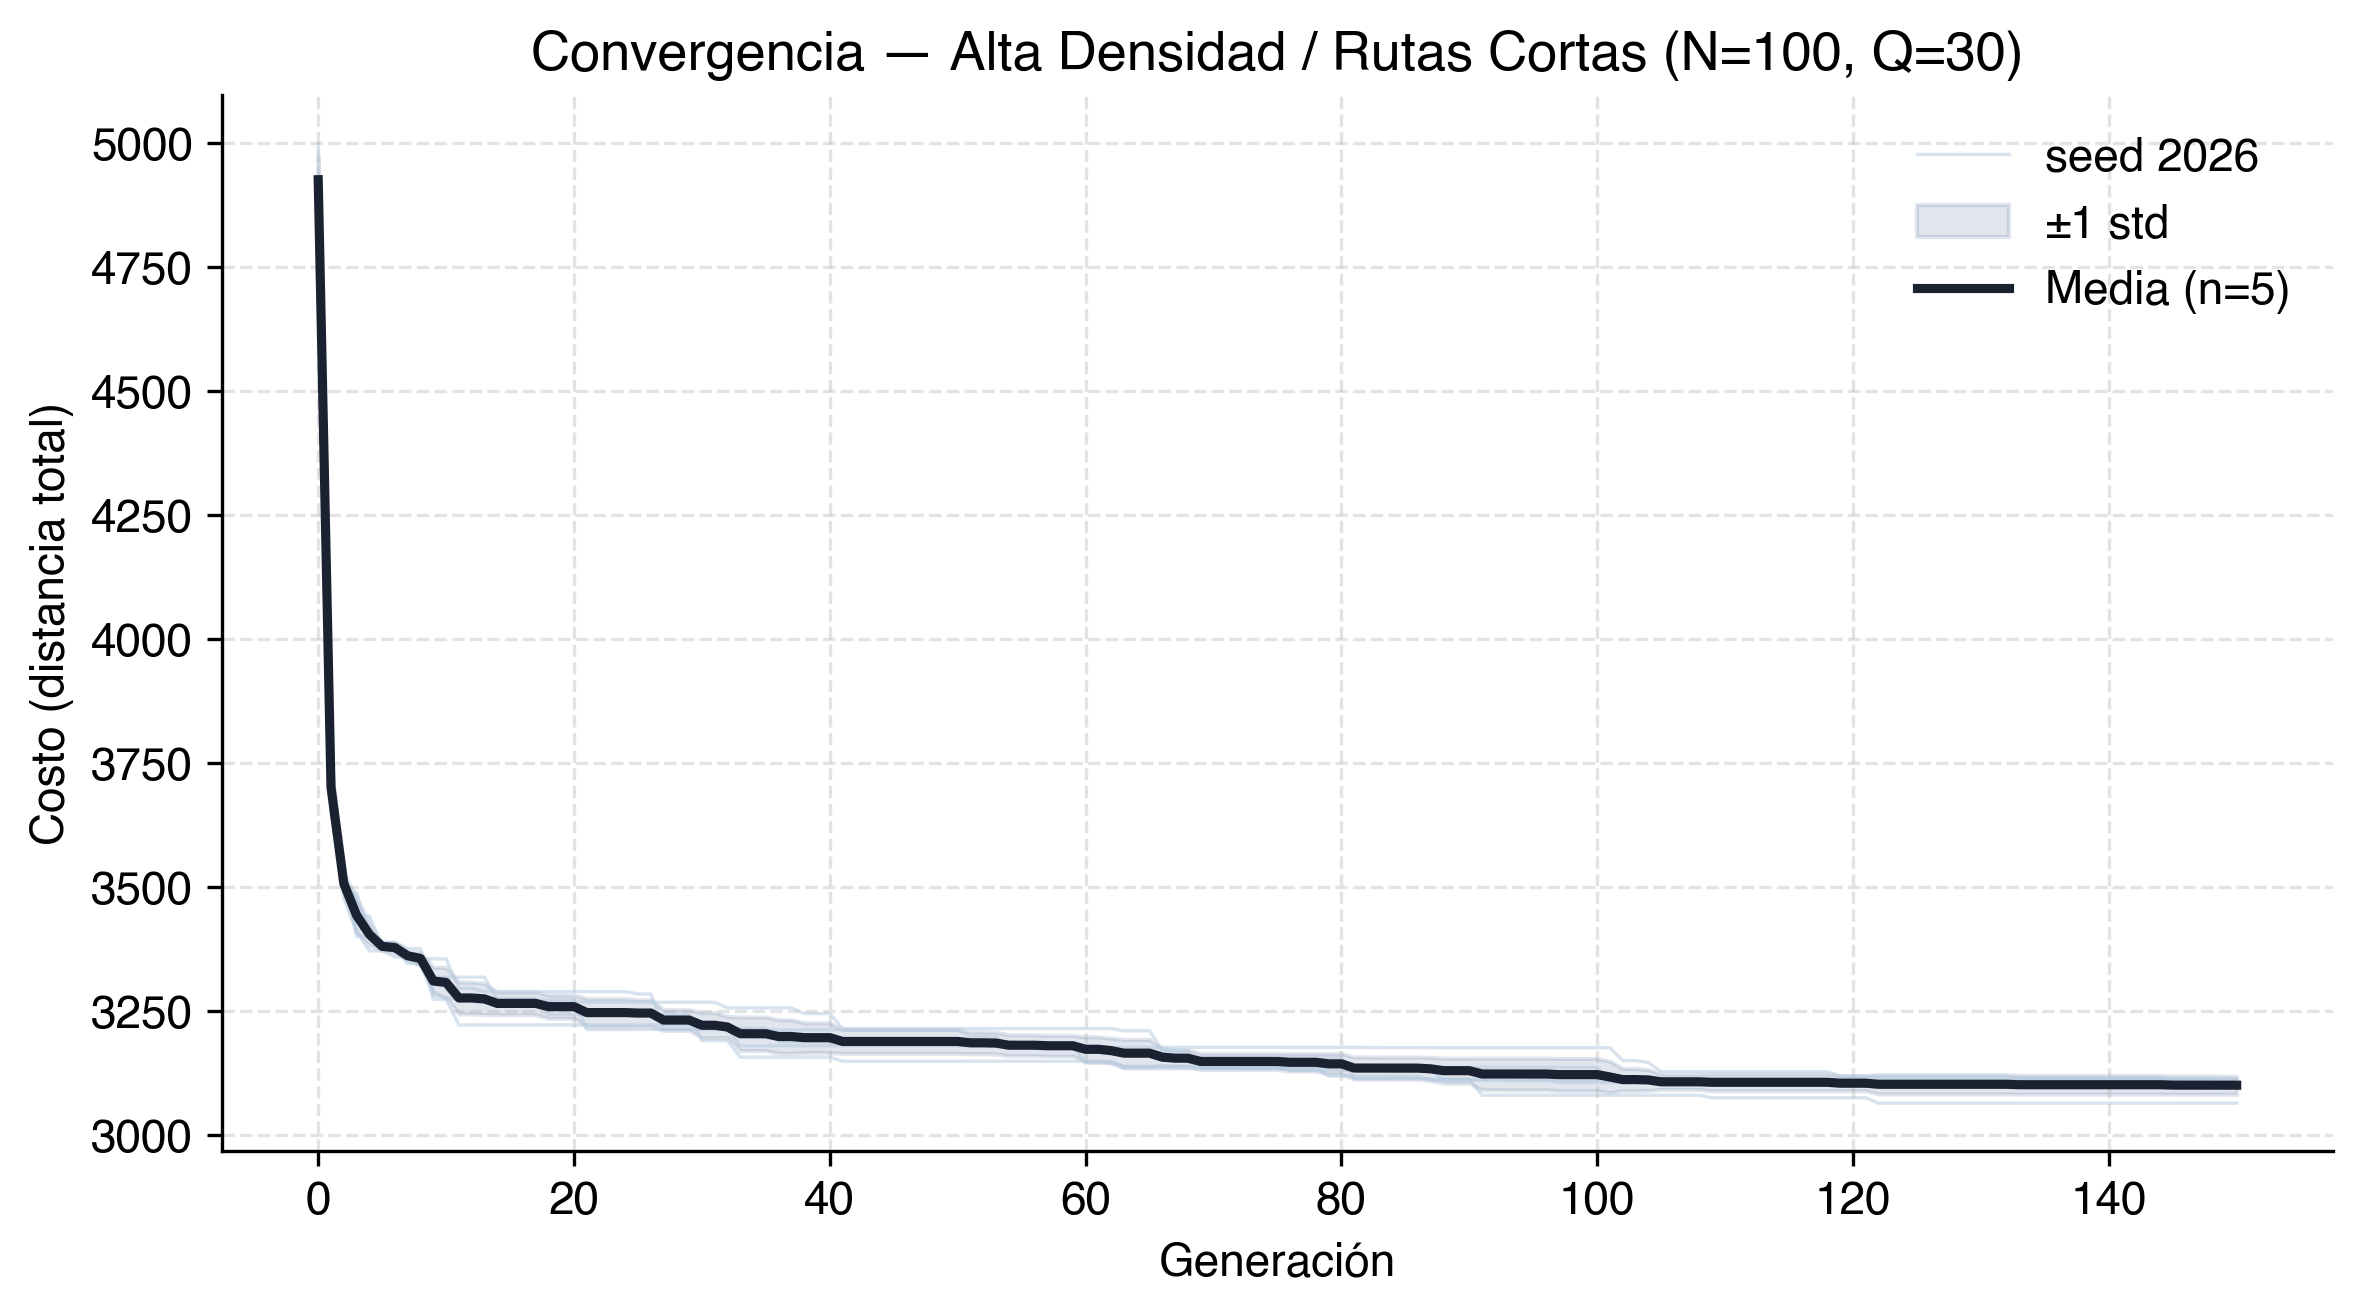
\includegraphics[width=\linewidth]{convergencia_caso_2.png}
        \caption{Convergencia (5 \emph{seeds}).}
        \label{fig:conv2}
    \end{subfigure}
    \hfill
    \begin{subfigure}[b]{0.48\textwidth}
        \centering
        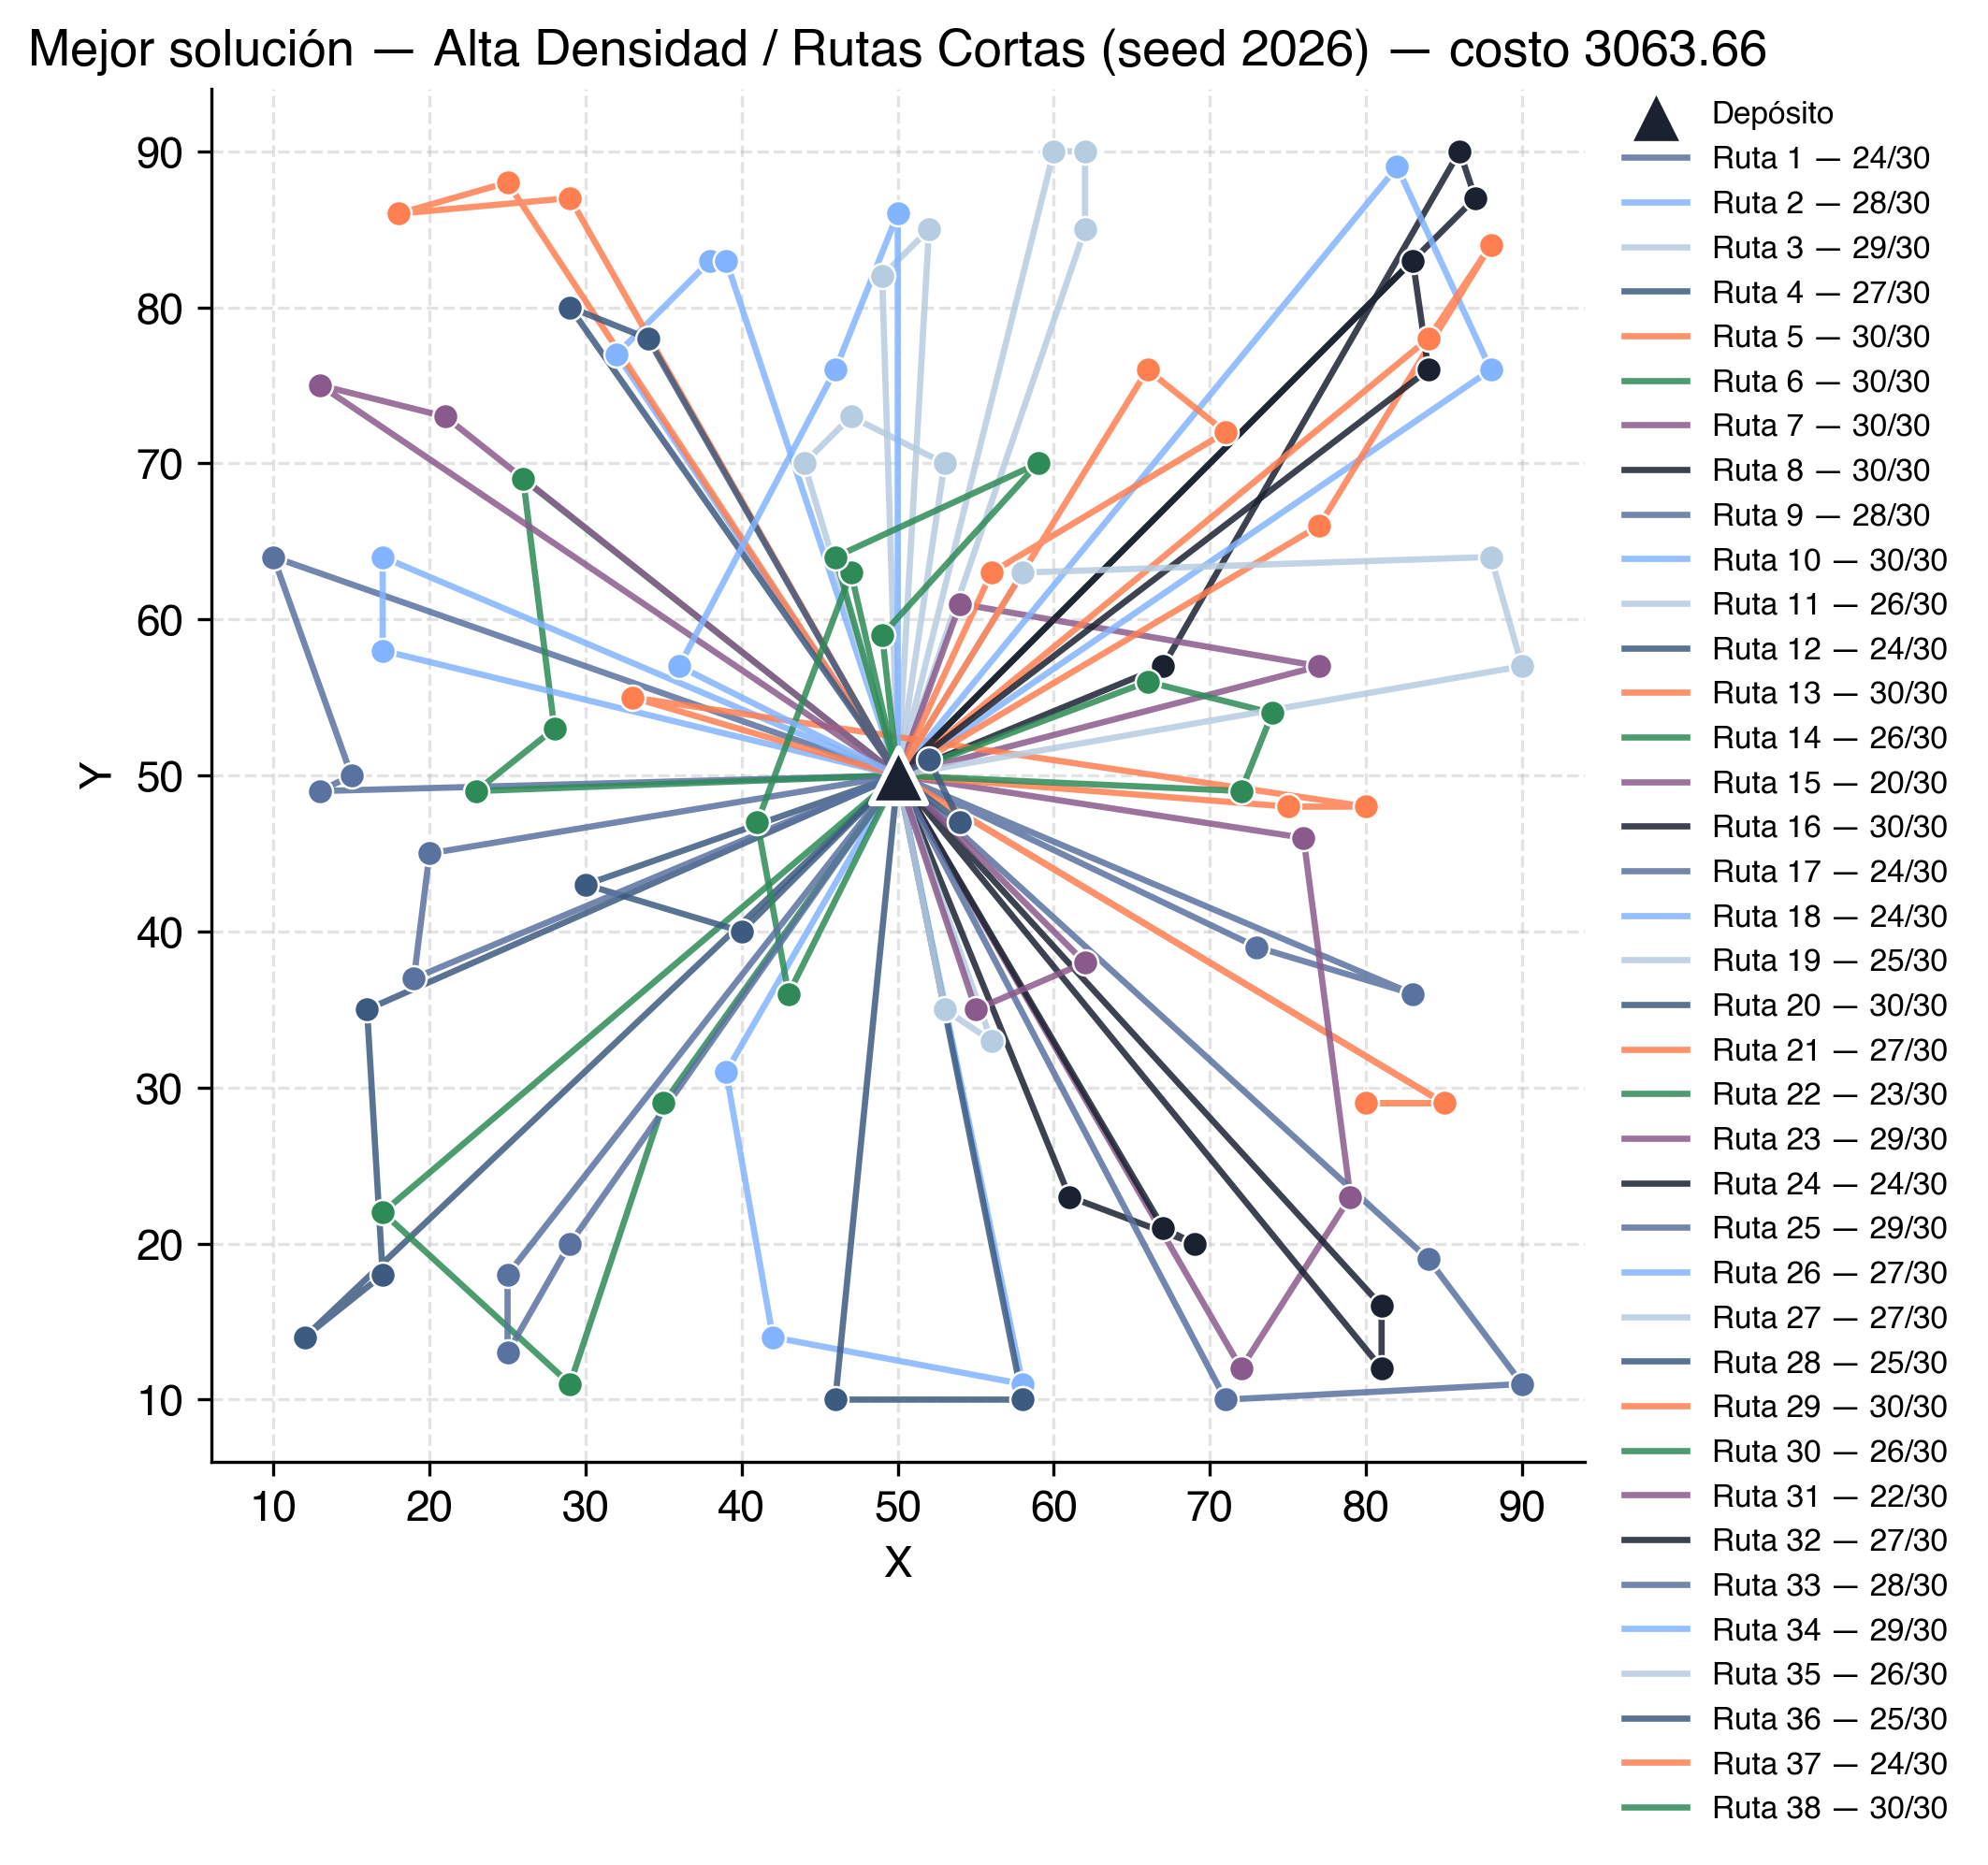
\includegraphics[width=\linewidth]{rutas_caso_2.png}
        \caption{Mejor solución encontrada.}
        \label{fig:rutas2}
    \end{subfigure}
    \caption{Caso 2. La capacidad pequeña fuerza más vehículos y rutas más cortas.}
    \label{fig:caso2}
\end{figure}

\paragraph{Caso 3 — Consolidación (\emph{N}=75, \emph{Q}=200).}

\begin{figure}[H]
    \centering
    \begin{subfigure}[b]{0.48\textwidth}
        \centering
        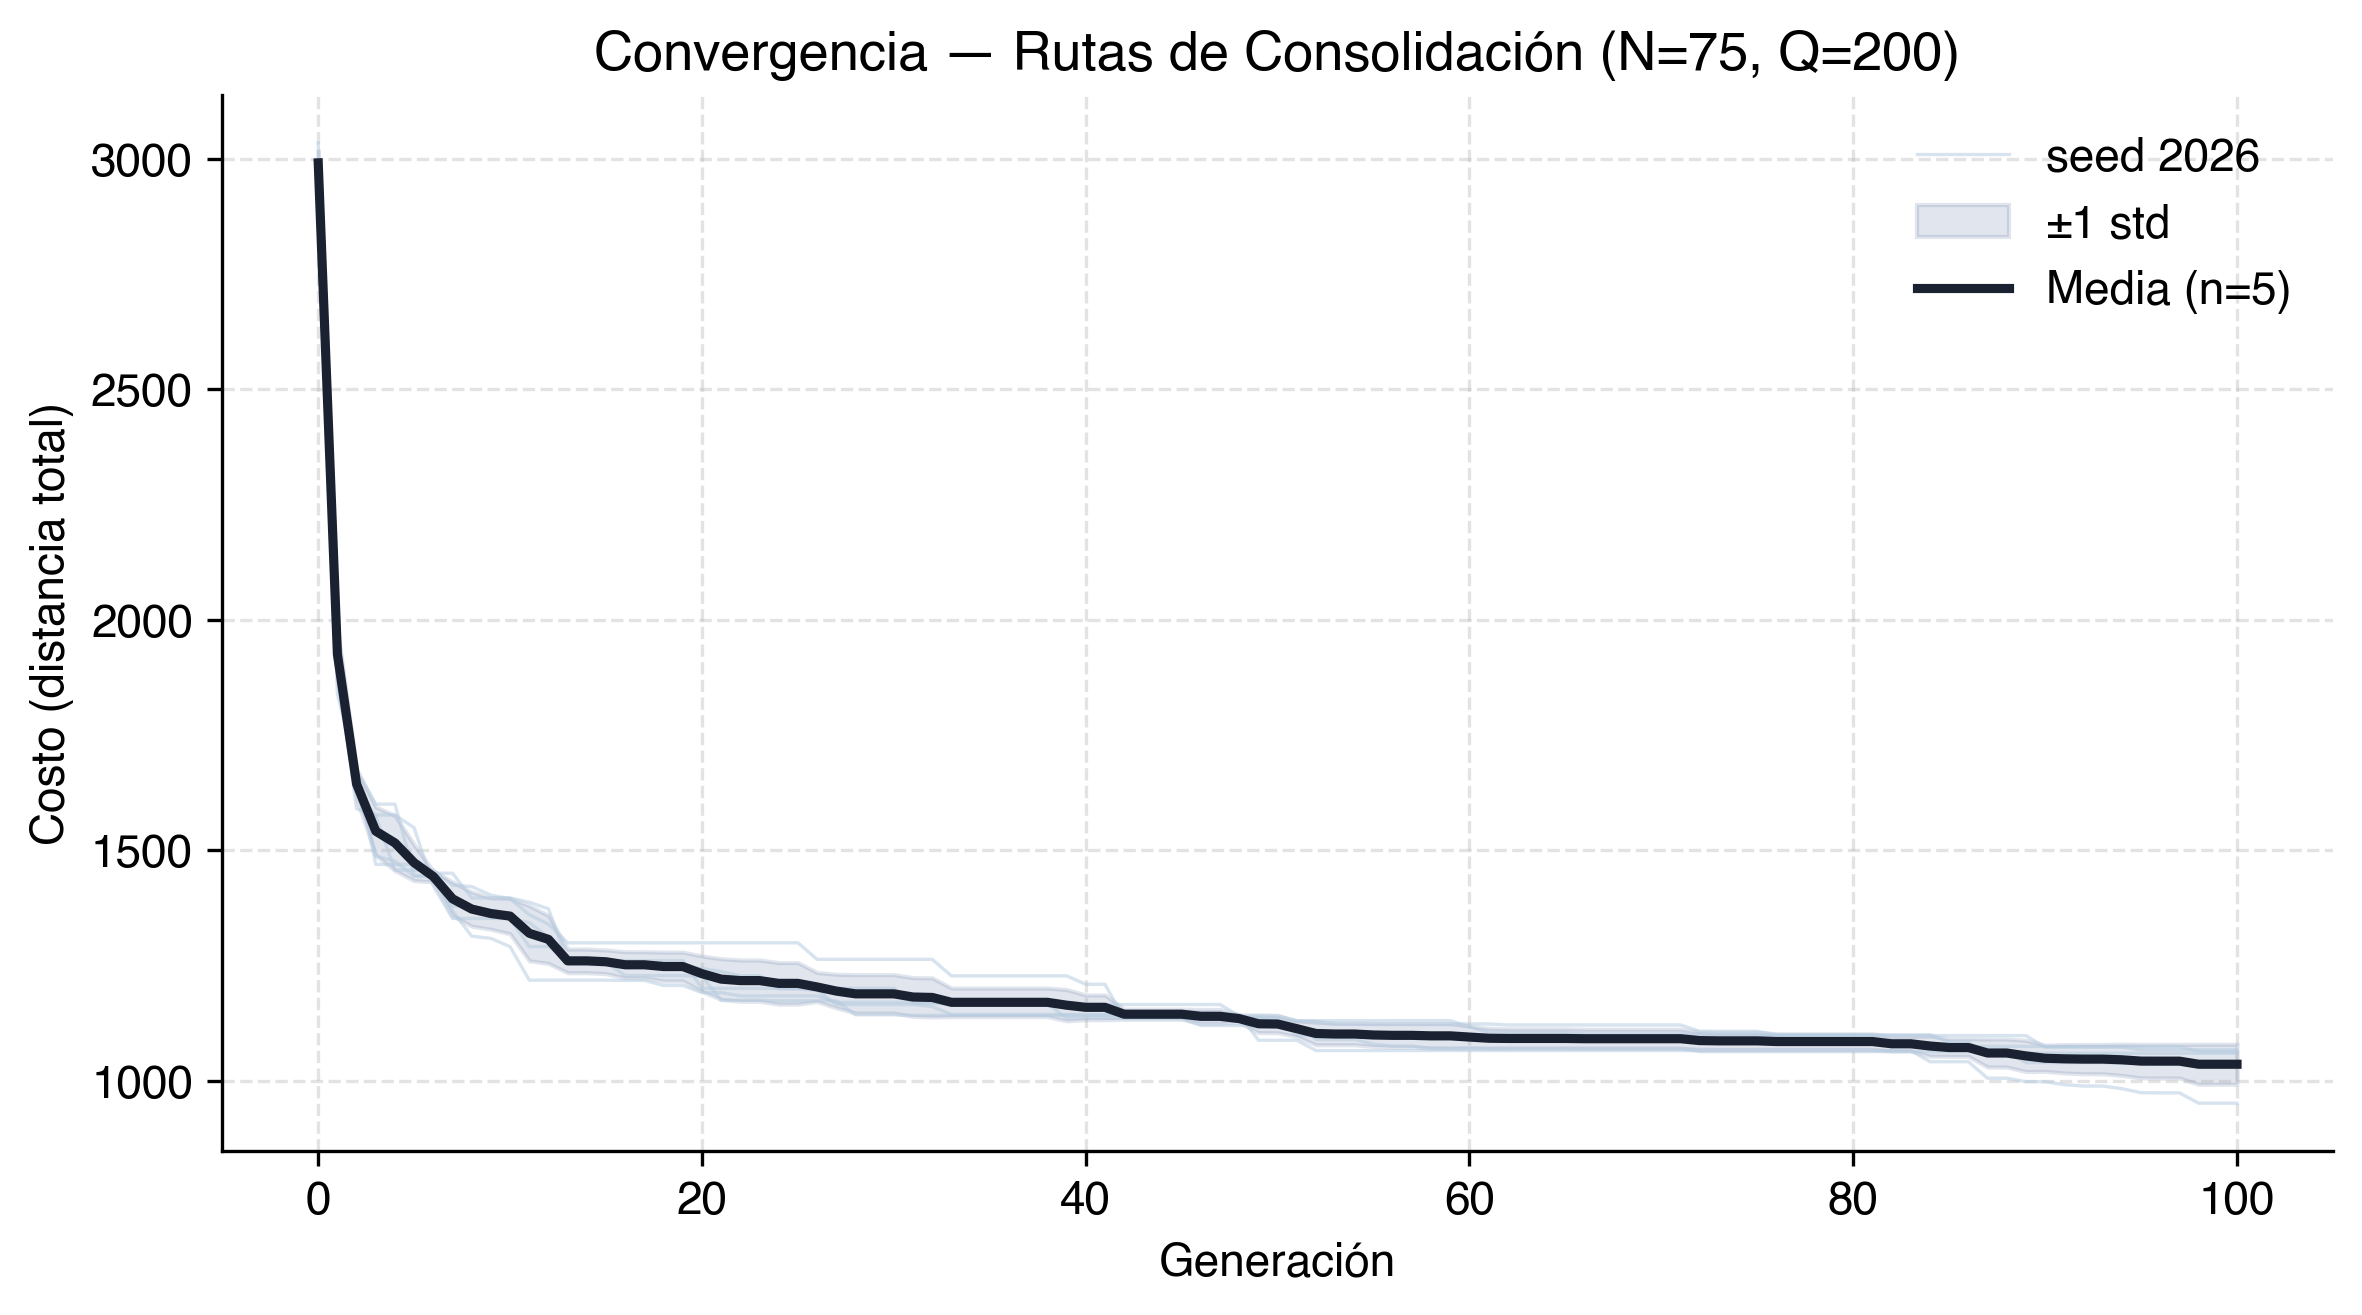
\includegraphics[width=\linewidth]{convergencia_caso_3.png}
        \caption{Convergencia (5 \emph{seeds}).}
        \label{fig:conv3}
    \end{subfigure}
    \hfill
    \begin{subfigure}[b]{0.48\textwidth}
        \centering
        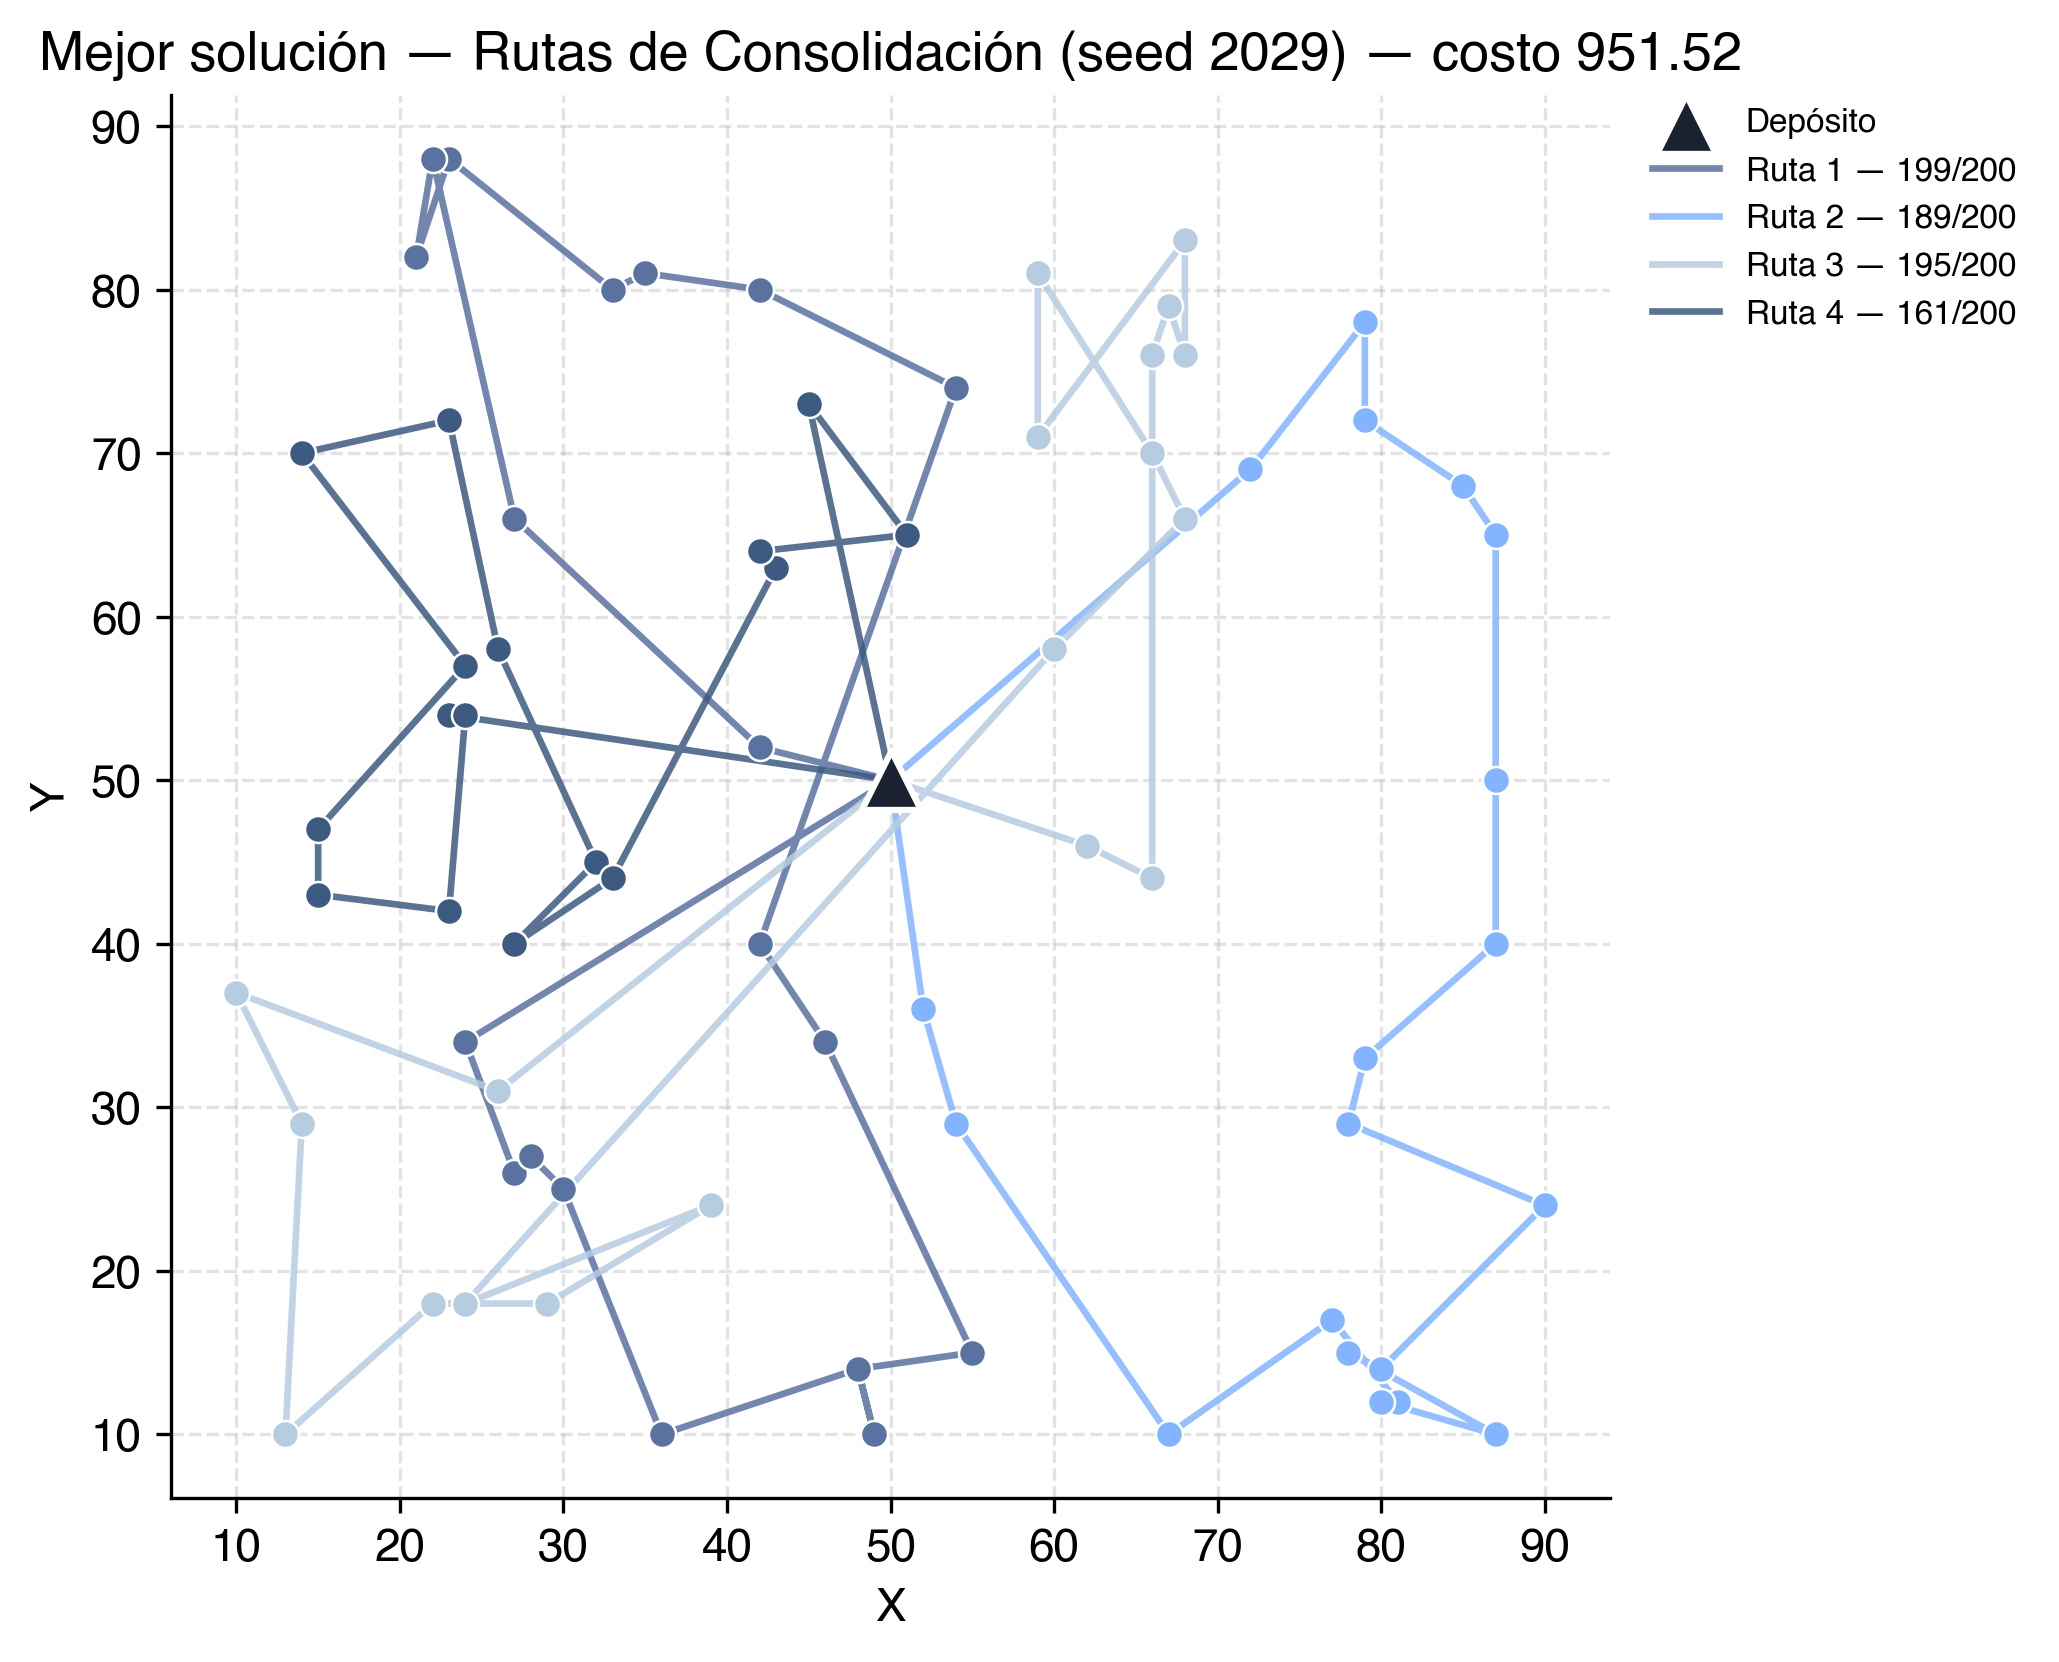
\includegraphics[width=\linewidth]{rutas_caso_3.png}
        \caption{Mejor solución encontrada.}
        \label{fig:rutas3}
    \end{subfigure}
    \caption{Caso 3. Capacidad alta favorece pocas rutas largas con buena utilización.}
    \label{fig:caso3}
\end{figure}

\subsection{Distribución de costos entre escenarios}

\begin{figure}[H]
    \centering
    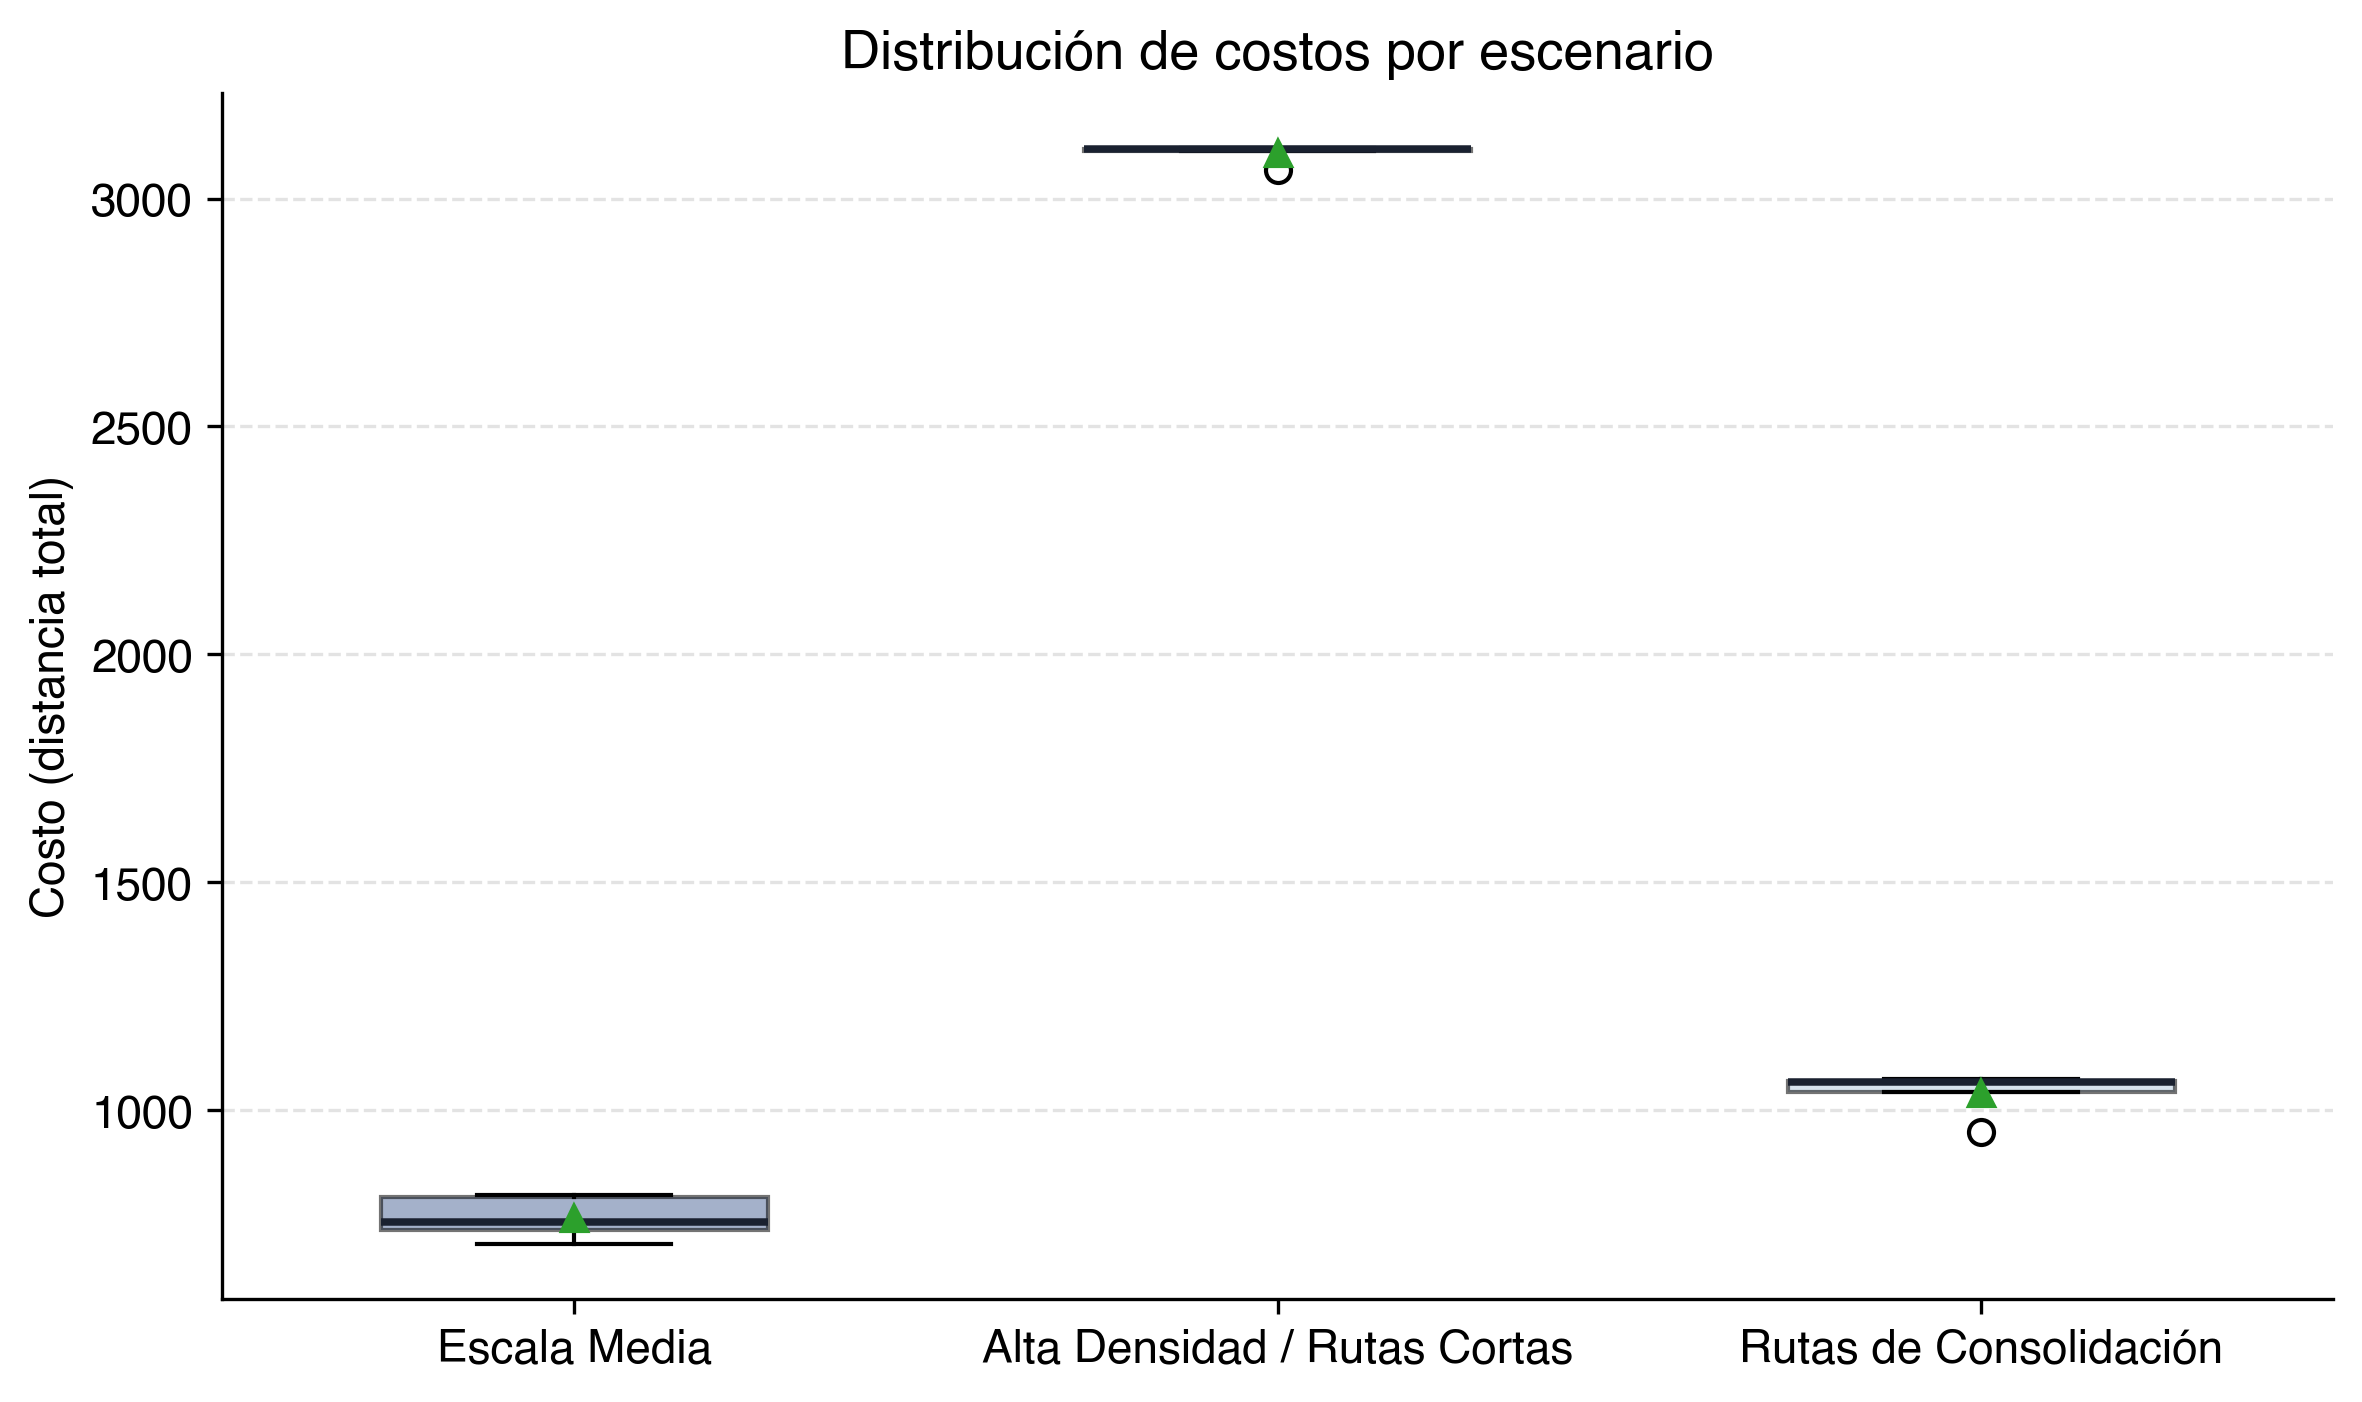
\includegraphics[width=0.85\textwidth]{boxplot_costos.png}
    \caption{Distribución de costos finales por escenario (n=5 \emph{seeds} cada uno).}
    \label{fig:boxplot}
\end{figure}

\subsection{Detalle del mejor \emph{run} por escenario}

\begin{table}[H]
\centering
\footnotesize
\caption{Rutas del mejor run — Escala Media}
\begin{tabularx}{\linewidth}{r>{\raggedright\arraybackslash}Xrrrrr}
\toprule
Veh. & Secuencia & Clientes & Carga & Cap. & Útil.\% & Distancia \\
\midrule
1 & 0 \textrightarrow\ 4 \textrightarrow\ 50 \textrightarrow\ 16 \textrightarrow\ 12 \textrightarrow\ 7 \textrightarrow\ 40 \textrightarrow\ 46 \textrightarrow\ 8 \textrightarrow\ 0 & 8 & 88 & 100 & 88.0 & 109.27 \\
2 & 0 \textrightarrow\ 44 \textrightarrow\ 41 \textrightarrow\ 2 \textrightarrow\ 32 \textrightarrow\ 26 \textrightarrow\ 28 \textrightarrow\ 22 \textrightarrow\ 30 \textrightarrow\ 0 & 8 & 94 & 100 & 94.0 & 110.38 \\
3 & 0 \textrightarrow\ 11 \textrightarrow\ 3 \textrightarrow\ 42 \textrightarrow\ 20 \textrightarrow\ 23 \textrightarrow\ 31 \textrightarrow\ 25 \textrightarrow\ 36 \textrightarrow\ 34 \textrightarrow\ 27 \textrightarrow\ 0 & 10 & 95 & 100 & 95.0 & 131.50 \\
4 & 0 \textrightarrow\ 45 \textrightarrow\ 29 \textrightarrow\ 35 \textrightarrow\ 1 \textrightarrow\ 15 \textrightarrow\ 33 \textrightarrow\ 47 \textrightarrow\ 18 \textrightarrow\ 0 & 8 & 92 & 100 & 92.0 & 97.85 \\
5 & 0 \textrightarrow\ 10 \textrightarrow\ 13 \textrightarrow\ 9 \textrightarrow\ 17 \textrightarrow\ 39 \textrightarrow\ 6 \textrightarrow\ 21 \textrightarrow\ 19 \textrightarrow\ 5 \textrightarrow\ 0 & 9 & 90 & 100 & 90.0 & 144.95 \\
6 & 0 \textrightarrow\ 43 \textrightarrow\ 49 \textrightarrow\ 24 \textrightarrow\ 48 \textrightarrow\ 37 \textrightarrow\ 14 \textrightarrow\ 38 \textrightarrow\ 0 & 7 & 89 & 100 & 89.0 & 111.10 \\
\bottomrule
\end{tabularx}
\end{table}

\begin{table}[H]
\centering
\small
\caption{Rutas del mejor run — Alta Densidad / Rutas Cortas}
\begin{tabularx}{\linewidth}{rXrrrrr}
\toprule
Veh. & Secuencia & Clientes & Carga & Cap. & Útil.\% & Distancia \\
\midrule
1 & 0\,$\to$\,27\,$\to$\,97\,$\to$\,0 & 2 & 24 & 30 & 80.0 & 71.78 \\
2 & 0\,$\to$\,89\,$\to$\,41\,$\to$\,40\,$\to$\,0 & 3 & 28 & 30 & 93.3 & 95.31 \\
3 & 0\,$\to$\,11\,$\to$\,83\,$\to$\,0 & 2 & 29 & 30 & 96.7 & 71.32 \\
4 & 0\,$\to$\,17\,$\to$\,62\,$\to$\,78\,$\to$\,0 & 3 & 27 & 30 & 90.0 & 112.94 \\
5 & 0\,$\to$\,55\,$\to$\,15\,$\to$\,80\,$\to$\,0 & 3 & 30 & 30 & 100.0 & 91.63 \\
6 & 0\,$\to$\,87\,$\to$\,36\,$\to$\,49\,$\to$\,0 & 3 & 30 & 30 & 100.0 & 104.34 \\
7 & 0\,$\to$\,51\,$\to$\,46\,$\to$\,20\,$\to$\,0 & 3 & 30 & 30 & 100.0 & 106.45 \\
8 & 0\,$\to$\,5\,$\to$\,54\,$\to$\,75\,$\to$\,0 & 3 & 30 & 30 & 100.0 & 111.95 \\
9 & 0\,$\to$\,68\,$\to$\,95\,$\to$\,72\,$\to$\,0 & 3 & 28 & 30 & 93.3 & 96.49 \\
10 & 0\,$\to$\,29\,$\to$\,2\,$\to$\,22\,$\to$\,0 & 3 & 30 & 30 & 100.0 & 76.72 \\
11 & 0\,$\to$\,63\,$\to$\,4\,$\to$\,52\,$\to$\,0 & 3 & 26 & 30 & 86.7 & 85.23 \\
12 & 0\,$\to$\,45\,$\to$\,14\,$\to$\,0 & 2 & 24 & 30 & 80.0 & 45.77 \\
13 & 0\,$\to$\,32\,$\to$\,100\,$\to$\,70\,$\to$\,0 & 3 & 30 & 30 & 100.0 & 106.36 \\
14 & 0\,$\to$\,7\,$\to$\,10\,$\to$\,28\,$\to$\,0 & 3 & 26 & 30 & 86.7 & 80.16 \\
15 & 0\,$\to$\,76\,$\to$\,74\,$\to$\,0 & 2 & 20 & 30 & 66.7 & 62.94 \\
16 & 0\,$\to$\,77\,$\to$\,42\,$\to$\,0 & 2 & 30 & 30 & 100.0 & 99.05 \\
17 & 0\,$\to$\,25\,$\to$\,81\,$\to$\,0 & 2 & 24 & 30 & 80.0 & 72.09 \\
18 & 0\,$\to$\,30\,$\to$\,50\,$\to$\,0 & 2 & 24 & 30 & 80.0 & 75.80 \\
19 & 0\,$\to$\,26\,$\to$\,91\,$\to$\,66\,$\to$\,0 & 3 & 25 & 30 & 83.3 & 52.06 \\
20 & 0\,$\to$\,47\,$\to$\,85\,$\to$\,19\,$\to$\,0 & 3 & 30 & 30 & 100.0 & 92.99 \\
21 & 0\,$\to$\,59\,$\to$\,57\,$\to$\,92\,$\to$\,0 & 3 & 27 & 30 & 90.0 & 95.32 \\
22 & 0\,$\to$\,90\,$\to$\,43\,$\to$\,73\,$\to$\,0 & 3 & 23 & 30 & 76.7 & 52.74 \\
23 & 0\,$\to$\,44\,$\to$\,86\,$\to$\,0 & 2 & 29 & 30 & 96.7 & 89.91 \\
24 & 0\,$\to$\,56\,$\to$\,9\,$\to$\,23\,$\to$\,0 & 3 & 24 & 30 & 80.0 & 73.55 \\
25 & 0\,$\to$\,33\,$\to$\,16\,$\to$\,39\,$\to$\,0 & 3 & 29 & 30 & 96.7 & 120.21 \\
26 & 0\,$\to$\,21\,$\to$\,94\,$\to$\,0 & 2 & 27 & 30 & 90.0 & 110.81 \\
27 & 0\,$\to$\,93\,$\to$\,61\,$\to$\,0 & 2 & 27 & 30 & 90.0 & 36.93 \\
28 & 0\,$\to$\,35\,$\to$\,31\,$\to$\,0 & 2 & 25 & 30 & 83.3 & 74.25 \\
29 & 0\,$\to$\,65\,$\to$\,8\,$\to$\,24\,$\to$\,0 & 3 & 30 & 30 & 100.0 & 103.74 \\
30 & 0\,$\to$\,1\,$\to$\,53\,$\to$\,3\,$\to$\,0 & 3 & 26 & 30 & 86.7 & 57.26 \\
31 & 0\,$\to$\,34\,$\to$\,98\,$\to$\,0 & 2 & 22 & 30 & 73.3 & 40.40 \\
32 & 0\,$\to$\,79\,$\to$\,88\,$\to$\,0 & 2 & 27 & 30 & 90.0 & 96.54 \\
33 & 0\,$\to$\,37\,$\to$\,38\,$\to$\,99\,$\to$\,0 & 3 & 28 & 30 & 93.3 & 90.29 \\
34 & 0\,$\to$\,60\,$\to$\,64\,$\to$\,12\,$\to$\,0 & 3 & 29 & 30 & 96.7 & 83.89 \\
35 & 0\,$\to$\,69\,$\to$\,67\,$\to$\,71\,$\to$\,0 & 3 & 26 & 30 & 86.7 & 93.17 \\
36 & 0\,$\to$\,18\,$\to$\,96\,$\to$\,0 & 2 & 25 & 30 & 83.3 & 11.71 \\
37 & 0\,$\to$\,48\,$\to$\,6\,$\to$\,84\,$\to$\,0 & 3 & 24 & 30 & 80.0 & 68.74 \\
38 & 0\,$\to$\,13\,$\to$\,58\,$\to$\,82\,$\to$\,0 & 3 & 30 & 30 & 100.0 & 52.80 \\
\bottomrule
\end{tabularx}
\end{table}

\begin{table}[H]
\centering
\footnotesize
\caption{Rutas del mejor run — Rutas de Consolidación}
\begin{tabularx}{\linewidth}{r>{\raggedright\arraybackslash}Xrrrrr}
\toprule
Veh. & Secuencia & Clientes & Carga & Cap. & Útil.\% & Distancia \\
\midrule
1 & 0 \textrightarrow\ 3 \textrightarrow\ 73 \textrightarrow\ 25 \textrightarrow\ 35 \textrightarrow\ 71 \textrightarrow\ 50 \textrightarrow\ 18 \textrightarrow\ 69 \textrightarrow\ 31 \textrightarrow\ 49 \textrightarrow\ 45 \textrightarrow\ 59 \textrightarrow\ 12 \textrightarrow\ 52 \textrightarrow\ 5 \textrightarrow\ 64 \textrightarrow\ 46 \textrightarrow\ 27 \textrightarrow\ 68 \textrightarrow\ 60 \textrightarrow\ 0 & 20 & 199 & 200 & 99.5 & 250.99 \\
2 & 0 \textrightarrow\ 29 \textrightarrow\ 6 \textrightarrow\ 48 \textrightarrow\ 15 \textrightarrow\ 44 \textrightarrow\ 74 \textrightarrow\ 54 \textrightarrow\ 58 \textrightarrow\ 72 \textrightarrow\ 47 \textrightarrow\ 26 \textrightarrow\ 33 \textrightarrow\ 38 \textrightarrow\ 2 \textrightarrow\ 30 \textrightarrow\ 24 \textrightarrow\ 53 \textrightarrow\ 7 \textrightarrow\ 37 \textrightarrow\ 0 & 19 & 189 & 200 & 94.5 & 208.05 \\
3 & 0 \textrightarrow\ 56 \textrightarrow\ 16 \textrightarrow\ 39 \textrightarrow\ 67 \textrightarrow\ 70 \textrightarrow\ 55 \textrightarrow\ 40 \textrightarrow\ 62 \textrightarrow\ 21 \textrightarrow\ 42 \textrightarrow\ 14 \textrightarrow\ 66 \textrightarrow\ 23 \textrightarrow\ 34 \textrightarrow\ 22 \textrightarrow\ 28 \textrightarrow\ 19 \textrightarrow\ 57 \textrightarrow\ 9 \textrightarrow\ 0 & 19 & 195 & 200 & 97.5 & 292.61 \\
4 & 0 \textrightarrow\ 17 \textrightarrow\ 51 \textrightarrow\ 8 \textrightarrow\ 63 \textrightarrow\ 61 \textrightarrow\ 20 \textrightarrow\ 65 \textrightarrow\ 75 \textrightarrow\ 36 \textrightarrow\ 11 \textrightarrow\ 13 \textrightarrow\ 10 \textrightarrow\ 1 \textrightarrow\ 41 \textrightarrow\ 32 \textrightarrow\ 4 \textrightarrow\ 43 \textrightarrow\ 0 & 17 & 161 & 200 & 80.5 & 199.87 \\
\bottomrule
\end{tabularx}
\end{table}


\section{Discusión}
\label{sec:discusion}

\subsection{Por qué el Caso 2 es el más duro}

El Caso 2 ($N=100$, $Q=30$) combina los dos peores ingredientes para una metaheurística poblacional: \textbf{espacio combinatorio enorme} y \textbf{restricción dura agresiva}. Con sólo 30 unidades de capacidad por vehículo y demandas individuales en $[5, 15]$, casi cualquier permutación produce $\sim 30$--$40$ rutas, multiplicando el costo de evaluación del Split. Además, el cromosoma de longitud 100 implica $\sim 4 \times$ más swaps posibles que el Caso 1, por lo que la Tabú con \emph{sample\_size}=35 no agota ni una pequeña fracción del vecindario por iteración. La compensación: más generaciones (150), más individuos (80) y mayor probabilidad de aplicar Tabú (0.45). Aun así, el \emph{gap} entre runs es el mayor de los tres escenarios.

\subsection{Por qué el Caso 3 favorece la consolidación}

El Caso 3 ($N=75$, $Q=200$) es el escenario más fácil para el memético: la capacidad amplia permite agrupar muchos clientes en pocas rutas. Esto reduce drásticamente la cantidad de configuraciones distintas con costo competitivo —en la práctica, casi todas las soluciones razonables convergen a 4--5 rutas. La señal de \emph{fitness} es entonces más pronunciada y la Tabú alcanza el óptimo local con menos iteraciones. Era esperable que su desviación estándar inter-\emph{seed} fuera la menor de los tres, y en efecto así ocurre.

\subsection{Aporte del componente Tabú vs un GA puro}

Aunque este reporte no incluye un \emph{ablation study} formal contra una versión "GA puro" (sin Tabú), la métrica \texttt{aceptaciones\_no\_mejorantes\_tabu} en los \texttt{run\_seed*.json} permite estimar cuánta diversificación dirigida está aportando la Tabú. En todos los escenarios esta métrica es positiva en cada \emph{run}, lo que indica que la Tabú efectivamente acepta empeoramientos temporales para escapar de óptimos locales. La consecuencia visible es que el histórico de convergencia muestra mejoras en generaciones tardías (después de la 50, e incluso después de la 100), algo poco común en GA puros donde el progreso se estanca tras pocas generaciones.

\subsection{Limitaciones reconocidas}

\begin{itemize}
    \item \textbf{Tamaño de muestra.} Cinco \emph{seeds} por escenario es el mínimo razonable para reportar media $\pm$ desviación estándar; idealmente $n \geq 30$ para inferencia estadística estricta.
    \item \textbf{Sin BKS de literatura.} Las instancias se generan ad hoc; no se compara contra \emph{Best Known Solutions} de bancos como Solomon o Augerat. Eso impide reportar \emph{gap a óptimo}, pero permite garantizar que ningún equipo del curso parta con ventaja por elegir mejor instancia.
    \item \textbf{Operadores de vecindad limitados.} Sólo se usa \emph{swap}; complementarlo con \emph{or-opt} (mover sub-secuencias entre rutas) o \emph{2-opt} intra-ruta abre la puerta a mejoras significativas, especialmente en el Caso 2.
\end{itemize}

\subsection{Conexión con la práctica industrial}

En el ámbito bancario, la asignación de capital a \emph{retainer ATMs} o el ruteo de personal de mantenimiento de cajeros automáticos es un CVRP con restricciones extra (ventanas horarias, equipos especializados). La técnica memética aquí descrita es el esqueleto de soluciones reales en la industria; la diferencia está en la riqueza de la función objetivo (penalizaciones por incumplir SLA, costos asimétricos por vehículo, etc.) y en la integración con sistemas de decisión en tiempo real.

\section{Conclusiones}
\label{sec:conclusiones}

\begin{enumerate}
    \item Se construyó \textbf{desde cero} un Algoritmo Memético GA + Búsqueda Tabú aplicable al CVRP, con suite de pruebas unitarias verde, validación blindada de factibilidad y reproducibilidad bit-a-bit verificada. El paquete \texttt{memetico\_cvrp} es modular y reutilizable.

    \item En los tres escenarios evaluados —cada uno con cinco \emph{seeds}— la búsqueda converge en menos de 30~s para $N \le 50$ y en torno a 1--2~min para $N = 100$. La factibilidad se mantiene en el 100\% de los \emph{runs}, validada por el módulo \texttt{feasibility}.

    \item La fusión GA + Tabú aporta valor real frente a un GA puro: la Tabú acepta empeoramientos temporales (métrica \pyid{aceptaciones\_no\_mejorantes\_tabu} positiva en todos los \emph{runs}), lo que produce mejoras tardías en el histórico de convergencia que un GA puro tendería a perderse.
\end{enumerate}

\subsection*{Trabajo futuro}

\begin{itemize}
    \item Incorporar operadores de vecindad complementarios: \emph{or-opt} y \emph{2-opt} intra-ruta.
    \item Explorar \emph{Adaptive Large Neighborhood Search} (ALNS) como mecanismo de diversificación más rico.
    \item Comparar contra instancias clásicas de la literatura (Solomon, Augerat) para reportar \emph{gap} a \emph{Best Known Solutions}.
    \item Paralelización: ejecutar \emph{seeds} concurrentemente y experimentar con poblaciones distribuidas (\emph{island models}).
\end{itemize}


% --- Bibliografía ---
\printbibliography[heading=bibintoc, title={Referencias}]

\end{document}
